% This is samplepaper.tex, a sample chapter demonstrating the
% LLNCS macro package for Springer Computer Science proceedings;
% Version 2.21 of 2022/01/12
%
\documentclass[a4paper,runningheads]{llncs}
%
\usepackage[T1]{fontenc}
\usepackage{graphicx}
\usepackage{amsmath}
\usepackage{amssymb}
\usepackage{booktabs}
\usepackage{multirow}
\usepackage[table]{xcolor}
\usepackage{xcolor}
\usepackage{bm}
\usepackage{subcaption}
\usepackage{float}
\usepackage{svg}
\usepackage{url}
\usepackage{microtype}
\setlength{\emergencystretch}{2em}
% Note: The titlesec package has been completely removed to avoid LLNCS template conflicts.

\def\mymethod{MFCD}
\definecolor{mybgc}{rgb}{0.9, 0.9, 0.9} % 定义我的绿色作为表格底色
\definecolor{myred}{RGB}{255,0,0}   % 自定义红色
\definecolor{mygreen}{RGB}{0,128,0} % 自定义绿色
\newcommand{\redbf}[1]{\textcolor{myred}{\textbf{#1}}} % 红色粗体
\newcommand{\red}[1]{\textcolor{myred}{#1}} % 红色粗体
\newcommand{\green}[1]{\textcolor{mygreen}{#1}}       % 绿色文本

\graphicspath{{./}{figures/}}

\titlerunning{A Dual-Stream Cognitive Diagnosis Framework}

\begin{document}

\title{A Dual-Stream Cognitive Diagnosis Framework via Mastery-Fluency Disentanglement}

\author{Jiacheng Yi\inst{1} \and
Xiaoyao Li\inst{1}$^{*}$ \and
Lianhong Wang\inst{2} \and
Gufeng Gong\inst{1} \and
Wei Xu\inst{1}}

\authorrunning{J. Yi et al.}

\institute{School of Advanced Interdisciplinary Studies, Central South University of Forestry and Technology, Changsha 410004, China
\and
College of Electrical and Information Engineering, Hunan University, Changsha 410082, China\\
\email{lxy0731@csuft.edu.cn}}

\maketitle

\begingroup
\renewcommand{\thefootnote}{\fnsymbol{footnote}}
\footnotetext[0]{$*$ Corresponding author.}
\endgroup

% ==============================================================================
% ABSTRACT
% ==============================================================================
\begin{abstract}
Cognitive diagnosis models traditionally estimate student proficiency solely from binary response correctness, which conflates conceptual mastery with procedural dynamics. This paper proposes \mymethod, a dual-stream cognitive diagnosis framework that disentangles mastery from fluency through multi-task learning. The cognitive stream adopts a standard CDM to produce base logits for cognitive mastery, while the behavioral stream extracts exposure intensity, empirical accuracy, and response consistency from historical interactions to capture behavioral fluency. A dynamic fusion gate is further applied to adaptively merge the two streams, and auxiliary reconstruction tasks preserve behavioral information in fluency representations via multi-task optimization. Extensive experiments on six benchmarks validate the effectiveness of \mymethod\ across various backbone models.

\keywords{Cognitive Diagnosis \and Behavioral Fluency \and Fusion Gate \and Multi-Task Optimization \and Educational Data Mining.}
\end{abstract}

% ==============================================================================
% 1. INTRODUCTION
% ==============================================================================
\section{Introduction}

Cognitive diagnosis (CD) is a fundamental task in educational data mining that aims to evaluate students' latent cognitive states based on their historical learning interactions and assessment records, as shown in Figure \ref{fig:cd}.
As a core driving mechanism of intelligent tutoring systems and massive open online courses, Cognitive Diagnosis Models (CDMs) provide essential quantitative support for personalized learning recommendations, adaptive testing, and intelligent curriculum design \cite{thai2010recommender}.

CD research has evolved from traditional psychometric models to machine learning-based approaches, and more recently to deep learning-based architectures.
Psychometric-based models \cite{fan1998item,linden2000computerized,reckase2009multidimensional,delatorre2009dina} provide strong theoretical interpretability through explicit statistical modeling of cognitive states, but fail to capture complex learning dynamics due to rigid parametric assumptions.
Learning latent cognitive states from historical interaction logs in a data-driven manner, machine learning-based models \cite{MF,SVM,FuzzyCDF,MvCRF} typically rely on manually designed features and shallow architectures, whereas deep learning-based models \cite{wang2020neural,wang2022neuralcd,xu2025fairwisa} also leverage neural networks to automatically capture complex, non-linear dependencies.

\begin{figure}[t]
\centering
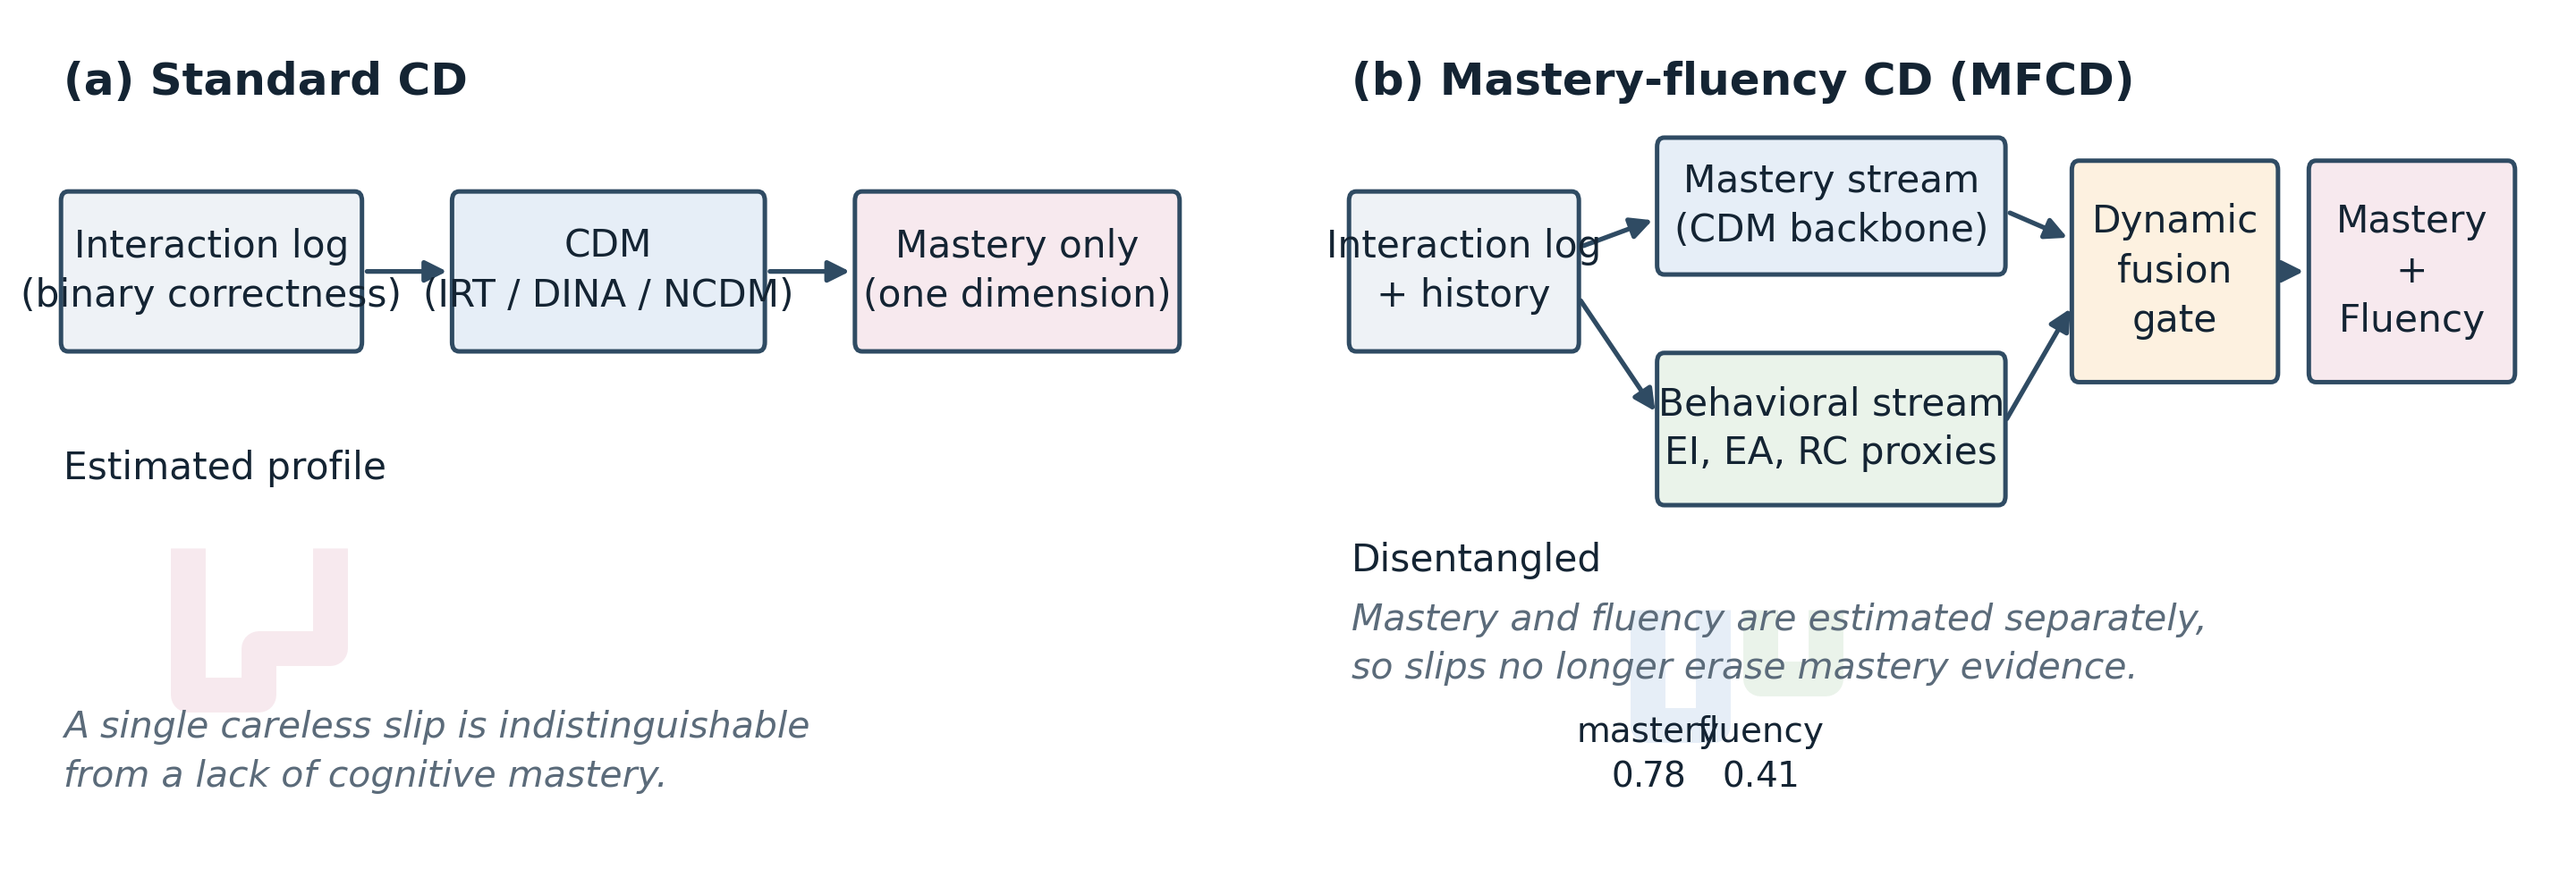
\includegraphics[width=\textwidth]{cd.png}
\caption{A toy example of typical CD and mastery-fluency CD.}
\label{fig:cd}
\end{figure}

% \begin{figure}[t]
% \centering
% \includesvg[width=\textwidth]{cd1}
% \caption{The flowchart of cognitive diagnosis.}
% \label{fig:cd}
% \end{figure}

As illustrated in the upper branch of Figure \ref{fig:cd}, the typical CD pipeline maps response logs to a unidimensional mastery profile, yielding only binary decisions such as mastered or non-mastered.
This diagnosis paradigm relies almost exclusively on binary correctness logs, reducing cognitive states to a single mastery dimension while overlooking the rich behavioral dynamics inherent in the learning process.
Pedagogy and cognitive psychology \cite{tenberge1999procedural} distinguish declarative knowledge (i.e., knowing a concept) from procedural knowledge (i.e., fluently solving a problem) as qualitatively distinct cognitive dimensions, and conflating a lack of fluency with a lack of mastery inevitably leads to biased diagnostic outcomes. For instance, a student may have fully understood fraction addition but still make a careless error. A traditional CDM would not only misdiagnose this as non-mastery but also trigger unnecessary interventions.

To overcome this limitation, as shown in the lower branch of Figure \ref{fig:cd}, we propose a paradigm shift from single-mastery diagnosis to joint modeling of mastery and fluency. Specifically, behavioral proxies (e.g., practice volume, historical accuracy, and response variability) are extracted from raw logs to build a fluency representation disentangled from cognitive mastery, enabling differentiated student state classification and precise, targeted interventions. To realize this paradigm, we propose \mymethod, a dual-stream framework that extends existing CDMs by disentangling cognitive mastery and behavioral fluency. Our main contributions are summarized as follows:
\vspace{-10pt}
\begin{itemize}
    \item We propose \mymethod, a novel and extensible CD framework that disentangles student profiles into mastery and fluency dimensions through  multi-task learning.
    \item We formalize three behavioral proxy features, namely exposure intensity, empirical accuracy and response consistency, and design a dynamic fusion gate to adaptively integrate behavioral fluency with cognitive mastery.
    \item Extensive evaluations on six benchmark datasets with various CDM baselines clearly demonstrate the rationale and effectiveness of our \mymethod.
\end{itemize}

% Despite continued algorithmic advances, most existing CDMs face notable limitations in practice. Their diagnoses rely almost exclusively on binary correctness logs, reducing cognitive states to a singular dimension of cognitive state, commonly referred to as knowledge mastery, while overlooking the rich behavioral dynamics inherent in the learning process. However, pedagogy and cognitive psychology \cite{smith1994misconceptions} distinguish declarative knowledge (i.e., knowing a concept) from procedural knowledge (i.e., fluently solving a problem) as qualitatively distinct cognitive dimensions. Therefore, conflating a lack of fluency with a lack of mastery inevitably leads to biased diagnostic outcomes. For example, a student may make a careless slip despite understanding fraction addition rules, and CDMs could not only misdiagnose this as non-mastery, but even trigger unnecessary interventions.

% Despite these algorithmic advancements, existing CDMs often face a critical bottleneck when deployed in real-world educational scenarios: they predominantly rely on binary correctness logs (i.e., whether a question was answered right or wrong) to estimate a singular, entangled dimension of cognitive state, commonly referred to as \textit{Knowledge Mastery}.
% Consequently, they structurally overlook the rich behavioral dynamics underlying the human learning process, such as problem-solving fluency, response stability over time, and incidental cognitive slips \cite{wang2024boosting,zhang2025cognitive}.

% From a pedagogical and cognitive psychology perspective, "knowing a concept" (declarative knowledge) and "fluently solving a problem" (procedural knowledge) are distinctly different cognitive dimensions \cite{smith1994misconceptions}.
% By conflating a "lack of fluency" with a "lack of mastery," traditional models tend to produce biased diagnostic reports.
% For instance, a student who fundamentally understands the abstract rules of fraction addition but makes a careless computational slip due to a low practice volume might be erroneously diagnosed by a standard NCDM as completely "unmastered" in the core concept.
% Such misdiagnoses inevitably lead to redundant pedagogical interventions, forcing students to re-watch basic theoretical lectures when all they truly need is targeted procedural practice to build muscle memory.
% Therefore, explicitly decoupling a student's cognitive state into distinct \textit{Mastery} and \textit{Fluency} dimensions is imperative for precise and high-resolution cognitive diagnosis.

% To directly address these challenges, we propose \textbf{\mymethod}, a novel Multi-Task Learning (MTL) framework designed to jointly model cognitive mastery and behavioral fluency.
% Our framework explicitly extracts and integrates behavioral proxy features to capture nuanced learning dynamics and employs an adaptive gating mechanism to dynamically fuse these dual states.
% Specifically, \mymethod\ constructs a secondary, independent behavioral module driven by three crucial mathematical proxy features: learning opportunity (the historical exposure rate to a specific concept), accuracy prior (historical correctness ratio reflecting empirical competence), and response stability (the statistical variance in student performance representing guessing or slipping).

% Furthermore, to dynamically integrate these features without suffering from the rigidity of static concatenation, we introduce an item-aware dynamic fusion gate mechanism.
% Rather than applying a fixed weight to behavioral features across all exercises indiscriminately, the gate self-adaptively evaluates the specific mathematical traits (difficulty and discrimination) of each given exercise.
% It dynamically calibrates the residual weights, allowing the model to rely heavily on the procedural fluency branch for repetitive, low-difficulty calculation tasks, while reverting to the fundamental mastery branch for complex, highly conceptual word problems.



% ==============================================================================
% 2. RELATED WORK
% ==============================================================================
\section{Related Work}

\subsection{Psychometrics-based CDMs}
Traditional psychometric-based CDMs can be categorized into ability-level and cognition-level paradigms. The ability-level paradigm focuses on macro-level holistic evaluation, modeling a student's overall ability as a continuous latent trait to predict response probability, without explicitly diagnosing specific knowledge components. Examples include Item Response Theory (IRT) \cite{fan1998item} and its multidimensional extension (MIRT) \cite{reckase2009multidimensional}, which characterize exercises via parameters such as discrimination, difficulty and guessing. In contrast, the cognition-level paradigm adopts a micro-level diagnostic perspective, modeling a student's knowledge state as a fine-grained binary attribute vector (i.e., mastered or not mastered) over specific knowledge concepts, as defined by the Q-matrix. For example, the Deterministic Input, Noisy "And" gate (DINA) model ~\cite{delatorre2009dina,delatorre2011generalized} assumes that a correct response requires mastery of all concepts associated with the exercise.

Despite their theoretical interpretability, these traditional CDMs are often too rigid to capture complex and non-linear learning trajectories, and their parametric assumptions further constrain adaptability to high-dimensional interaction data.

% The ability level paradigm is exemplified by Item Response Theory (IRT)\cite{fan1998item} and its multidimensional extension (MIRT)\cite{reckase2009multidimensional}, focuses on macro-level holistic evaluation. It aims to answer the question of "how strong is this student's overall ability" by modeling the probability of a correct response through a continuous latent ability variable. Parameters such as discrimination, difficulty, and guessing capture item characteristics, yet the output remains a global proficiency score without delving into specific knowledge structures. In contrast, the cognition level paradigm adopts a micro-level diagnostic perspective, addressing the more fundamental question: "Which specific knowledge points or skills has this student mastered, and where do the gaps remain?" The DINA model exemplifies this approach by representing a student's knowledge state as a binary attribute mastery vector, and explicitly employs a Q-matrix to specify the exact combination of skills required for each item. This fine-grained, attribute-level diagnosis provides actionable insights for targeted remediation, moving beyond the one-dimensional ability scores of traditional IRT frameworks.

% Cognitive Diagnosis Models (CDMs) have long been the cornerstone of personalized learning systems, designed to infer students' multidimensional latent traits from observable testing behaviors.
% Traditional psychometric approaches, such as Unidimensional and Multidimensional Item Response Theory (IRT, MIRT) \cite{fan1998item,reckase2009multidimensional}, along with cognitive diagnostic models like DINA \cite{delatorre2009dina}, typically rely on simple linear link functions or strict probabilistic mappings to model the interaction between student ability and item difficulty.
% While providing excellent statistical interpretability, these classical models are often too rigid to capture the complex, non-linear learning trajectories of modern online students.

\subsection{Learning-based CDMs}
In contrast to psychometrics-based models relying on strict theoretical assumptions, learning-based CDMs adopt a data-driven paradigm that directly learns latent cognitive states from historical interaction logs. These models are generally categorized into Machine Learning (ML)-based and Deep Learning (DL)-based approaches.

Early ML-based CDMs draw inspiration from collaborative filtering and matrix factorization, including matrix factorization~\cite{MF} and its probabilistic variant~\cite{PMF}, both of which factorize the student-exercise response matrix into low-dimensional latent trait vectors. Beyond matrix factorization, \cite{SVM} applies support vector machine to classify mastery states via maximum-margin hyperplanes. \cite{FuzzyCDF} employs a fuzzy set-theoretic framework that models continuous knowledge proficiency levels to accommodate both dichotomous and partially scored items. More recently, \cite{MvCRF} enriches cognitive profiling by extracting an effort trait from interaction logs, and integrating it with ability traits and a knowledge weakness parameter within a compensation mechanism.


DL-based CDMs leverage deep neural networks to automatically capture complex, non-linear interactions between students and exercises.
Neural CDM (NCDM)~\cite{wang2020neural} introduces a neural framework with non-negative layers to enforce educational monotonicity, ensuring both accuracy and interpretability.
To address sparse knowledge coverage, Knowledge-association based extension of the Neural Cognitive Diagnosis model (KaNCD)~\cite{wang2022neuralcd} models concept associations via low-dimensional embeddings, while Knowledge Concept Cold-Start Cognitive Diagnosis model (KCSCD)~\cite{zhang2026knowledge} targets concept cold-start via a gating-fused inference and ability module.
Beyond accuracy improvement, CD research has also expanded to other critical issues, such as fairness. The Fair cognitive diagnosis WIthout Sensitive Attributes (FairWISA)~\cite{xu2025fairwisa} is a model-agnostic framework that mitigates unfairness without requiring sensitive attributes, via a max-min training strategy for pseudo-group inference and fairness regularization.
% More recently, Large Language Model (LLM) have been introduced into this field. For instance, Knowledge-enhanced Cognitive Diagnosis (KCD)~\cite{dong2025knowledge} is a model-agnostic framework that leverages LLMs to generate textual diagnoses and aligns semantic and behavioral spaces via contrastive learning for improved performance in cold-start scenarios.

% Models like the Neural Cognitive Diagnosis Model (NCDM)  and its generalized framework NeuralCD \cite{wang2022neuralcd} extract complex, non-linear interaction features while elegantly preserving diagnostic interpretability by enforcing monotonicity constraints through non-negative fully connected layers.

% Similarly, models like FuzzyCDF \cite{liu2018fuzzy} attempt to capture the inherent fuzziness and uncertainty of student mastery.
% Despite their remarkable success, these deep CDMs still predominantly rely on discrete binary correctness data.
% They inherently conflate a student's fundamental conceptual understanding with their procedural test-taking state, leaving a critical blind spot in high-resolution cognitive profiling.



% \subsection{Behavioral Dynamics in Educational Data Mining}
% In real-world e-learning environments, students generate a wealth of behavioral and temporal data far beyond mere correctness.
% % Recent literature in Knowledge Tracing (KT) has begun to explore auxiliary behavioral indicators \cite{piech2015deep}.
% For instance, Dynamic Cognitive Diagnosis models attempt to incorporate temporal priors and forgetting curves \cite{wang2023dynamic}.
% % while other frameworks utilize anomalous learning interaction detection to enhance dataset robustness \cite{ma2024hd}.
% Studies have also successfully integrated students' affective states, emotional feedback, and response times to boost diagnostic accuracy \cite{wang2024boosting}.

% However, existing methodologies generally treat these temporal and behavioral signals as simple auxiliary inputs that are directly concatenated with cognitive embeddings before passing through a Multi-Layer Perceptron (MLP).
% From a cognitive perspective, this flat, static integration fails to theoretically decouple "Knowing" from "Doing" \cite{smith1994misconceptions}.
% A psychologically sound and highly interpretable framework requires explicitly encoding these historical behaviors into an independent latent procedural fluency state.

% \subsection{Feature Fusion and Adaptive Gating Mechanisms}
% Effectively combining multi-dimensional, heterogeneous features remains a persistent challenge in EDM.
% Recent advancements in explicit concept relation modeling and graph neural networks \cite{zhang2021gkt,su2022graph} have shown the immense benefits of structural priors.
% % Furthermore, models aiming for predictive, scalable, and interpretable tracing often rely on adaptive weighting \cite{zhou2024predictive,huang2024xkt}.
% Static fusion methods force the model to apply a rigid, unyielding set of weights to auxiliary features across all items, leading to severe feature entanglement.
% Implementing an adaptive gate network allows for the dynamic, item-specific weighting of fluency representations against mastery representations, ensuring that the diagnostic outcomes remain both highly accurate and profoundly explainable \cite{dong2025knowledge}.


% ==============================================================================
% 3. PROBLEM FORMULATION
% ==============================================================================
\section{Problem Formulation}

Let $\mathcal{U} = \{u_1, u_2, \dots, u_N\}$ denote the set of $N$ students, and $\mathcal{E} = \{e_1, e_2, \dots, e_M\}$ denote the set of $M$ exercises, $\mathcal{C} = \{c_1, c_2, \dots, c_K\}$ denote the set of $K$ knowledge concepts, and $\mathcal{R}=\{(u_i,e_j,r_{i,j})\mid u_i\in\mathcal{U}, e_j\in\mathcal{E}\}$ denote the set of response records, where binary response $r_{i,j}$ equals 0 for an incorrect answer or 1 for a correct answer.
The exercise-concept correlation matrix is encoded by a binary matrix named the Q-matrix, denoted as $\bm{Q}=[q_{j,k}]_{M \times K}$. Specifically, $q_{j,k}=1$ if concept $c_k$ is required to correctly answer item $e_j$, and $q_{j,k}=0$ otherwise.

\begin{definition}\label{def:cd}
(Cognitive Diagnosis) Given the response records $\mathcal{R}$ and the Q-matrix $\bm{Q}$, cognitive diagnosis aims to estimate students' latent cognitive states from their interaction histories. These states are typically represented by knowledge proficiency $\alpha_{i,k}$ of student $u_i \in \mathcal{U}$ on concept $c_k \in \mathcal{C}$, along with auxiliary item parameters such as difficulty and discrimination.
\end{definition}

\begin{definition}\label{def:ddgs}
Difficulty and discrimination parameters characterize exercise properties, and guessing and slip parameters capture inconsistencies between observed responses and latent cognitive states.
Difficulty quantifies the baseline success probability for an average-proficiency student.
Discrimination measures how sensitively the success probability responds to changes in cognitive states.
Guessing quantifies the probability of a correct response despite lacking the corresponding knowledge state.
Slip measures the probability of an incorrect response despite possessing the corresponding knowledge state.
\end{definition}

For each exercise $e_j\in\mathcal{E}$, its difficulty, discrimination guessing and slip parameters are typically denoted as $\bm{h}_j^{\text{diff}}, \bm{h}_j^{\text{disc}} \in \mathbb{R}^K, h_j^{\text{gues}}, h_j^{\text{slip}} \in \mathbb{R}$ ($j\in\{1,2,\cdots,M\}$), respectively.

% During the learning process, students continuously interact with exercises.
% The historical interaction sequence of a student $u$ up to time step $T$ can be represented as a chronologically ordered set of tuples:
% \begin{equation}
%     \mathcal{X}_u = \{(e_1, a_1), (e_2, a_2), \dots, (e_T, a_T)\}
% \end{equation}
% where $e_t \in \mathcal{E}$ is the exercise attempted at time step $t$, and $a_t \in \{0, 1\}$ denotes the binary response correctness score ($1$ for correct, $0$ for incorrect).

% \textbf{Objective:} Given the interaction history $\mathcal{X}_u$ of a student $u$ and the Q-matrix $Q$, the primary goal of a Cognitive Diagnosis Model is twofold:
% 1. To accurately predict the probability $P(a_{T+1} = 1 \mid u, e_{T+1})$ that student $u$ will answer a new target exercise $e_{T+1}$ correctly.
% 2. To infer an interpretable, multidimensional latent proficiency vector $h_u \in [0, 1]^K$, representing the student's mastery level over each specific knowledge concept in $\mathcal{K}$.


% ==============================================================================
% 4. METHODOLOGY
% ==============================================================================
\section{Methodology}

Figure \ref{fig:architecture} illustrates the overall architecture of \mymethod, which consists of mastery stream, behavioral stream, and dynamic fusion gate, jointly optimized under multi-task optimization to preserve behavioral information.

\begin{figure}[t]
\centering
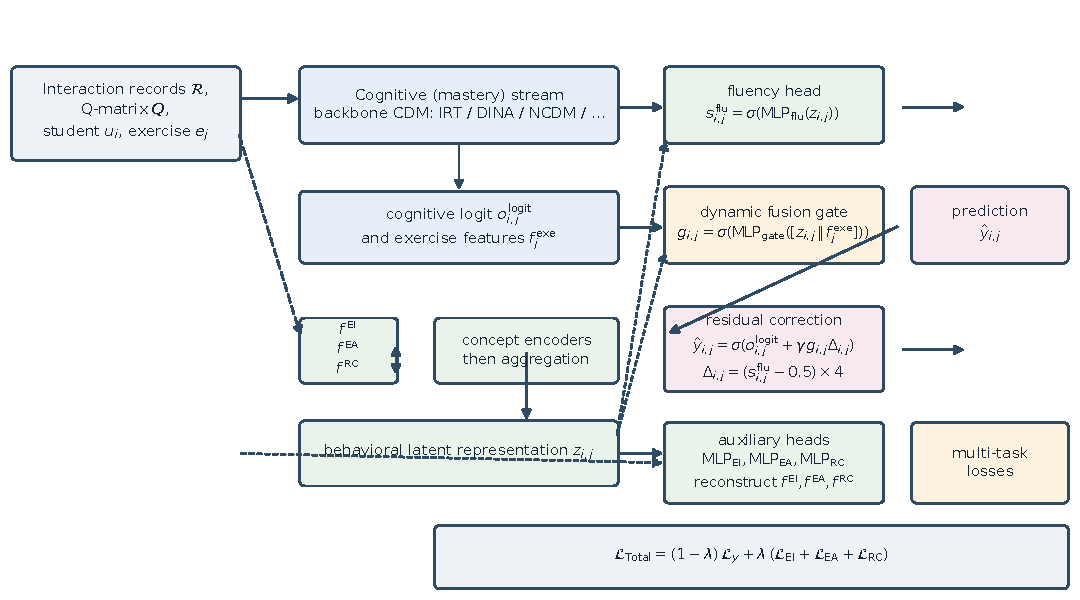
\includegraphics[width=\textwidth]{ours_flowchart.pdf}
\caption{The overall architecture of \mymethod.}
\label{fig:architecture}
\end{figure}

% \begin{figure}[t]
% \centering
% \includegraphics[width=\textwidth]{333.png}
% \caption{The overall architecture of \mymethod. The model processes inputs through a dual-stream design: the upper Mastery Backbone calculates fundamental cognitive competence via monotonicity-constrained layers, while the lower Behavioral Fluency Module extracts procedural familiarity. The two streams are adaptively merged via the Fusion Gate.}
% \label{fig:architecture}
% \end{figure}

\subsection{Cognitive Stream}
According to the core monotonicity assumption of CD, we adopt a standard CDM (e.g., NCDM, DINA, or IRT) as the cognitive stream, which takes the response records $\mathcal{R}$ and Q-matrix $\bm{Q}$ as input. For a given student $u_i$ and exercise $e_j$, the stream produces the mastery logit $o_{i,j}^{\text{logit}}$ of the base correct response probability as below:
\begin{equation}
    \left\{o_{i,j}^{\text{logit}}, \mathcal{F}_j \right\}= \text{CDM}\left(u_i,e_j,\mathcal{R},\bm{Q}\right)
\end{equation}
where $\mathcal{F}_j \subseteq \left\{\bm{h}_j^{\text{diff}}, \bm{h}_j^{\text{disc}}, h_j^{\text{gues}}, h_j^{\text{slip}},\cdots\right\}$ denotes the set of exercise-specific cognitive parameters provided by the standard CDM. For example, $\mathcal{F}_j = \left\{\bm{h}_j^{\text{diff}}, \bm{h}_j^{\text{disc}}\right\}$ for NCDM, and $\mathcal{F}_j = \left\{h_j^{\text{gues}}, h_j^{\text{slip}}\right\}$ for DINA.

\subsection{Behavioral Stream}
To capture procedural learning dynamics, we introduce three statistical behavioral features based on each student's historical interactions with each knowledge concept, namely exposure intensity, empirical accuracy and response consistency. Let $\mathcal{R}_{i,k} = \left\{\left(u_i, e_j, r_{i,j}\right) \mid \left(u_i, e_j, r_{i,j}\right) \in \mathcal{R}, \, q_{j,k} = 1\right\}$ denote the subset of historical records for student $u_i$ that are associated with concept $c_k$. These features are formalized using $\mathcal{R}_{i,k}$ as follows.

\begin{itemize}
    \item \textbf{Exposure Intensity} quantifies the cumulative interaction density of a student with a specific concept.
        \begin{equation}
        f_{i,k}^{\text{EI}} = \log\left(1 + |\mathcal{R}_{i,k}|\right)
        \end{equation}
    where $|\mathcal{R}_{i,k}|$ is the size of the record subset $\mathcal{R}_{i,k}$.

    \item \textbf{Empirical Accuracy} reflects the observed historical correctness rate.
        \begin{equation}
        f_{i,k}^{\text{EA}}  = \frac{\sum_{(u_i, e_j, r_{i,j}) \in \mathcal{R}_{i,k}} r_{i,j}}{|\mathcal{R}_{i,k}| + \epsilon}
        \end{equation}
    where $\epsilon$ is a small smoothing constant (e.g., $10^{-5}$) that prevents division by zero.

    \item \textbf{Response Consistency} measures the stability in the student's recent correctness pattern, capturing erratic behaviors indicative of slips or guesses.
        \begin{equation}
        f_{i,k}^{\text{RC}}  = 1-4\cdot \text{Var}\left(\left\{r_{i,j} \mid (u_i, e_j, r_{i,j}) \in \mathcal{R}_{i,k}\right\}\right)
        \end{equation}
    where $\text{Var}(\cdot)$ denotes the variance operator, measuring the dispersion of the correctness values.
\end{itemize}
Then, the above three behavioral features are concatenated and processed by a multi-layer perceptron (MLP) to obtain a latent fluency state $\bm{z}_{i,j}\in \mathbb{R}^D$:
\begin{equation}
    \bm{z}_{i,j} = \text{MLP}_{\text{beh}}\left(\left[f_{i,j}^{\text{EI}} \parallel f_{i,j}^{\text{EA}} \parallel f_{i,j}^{\text{RC}}\right] \right) + \tanh\left(\bm{b}_{u_i}\right)
\end{equation}
where $\bm{b}_{u_i} \in \mathbb{R}^D$ is a learnable student-specific bias term that captures the intrinsic fluency tendency of student $u_i$, independent of the current exercise context.
Here,
\begin{align}
&f_{i,j}^{\text{EI}} = \text{Agg}\left(\left\{f_{i,k}^{\text{EI}} \bigm| \ q_{j,k} = 1, k \in \{1,\dots,K\}\right\}\right),\\
&f_{i,j}^{\text{EA}} = \text{Agg}\left(\left\{f_{i,k}^{\text{EA}} \bigm| \ q_{j,k} = 1, k \in \{1,\dots,K\}\right\}\right),\\
&f_{i,j}^{\text{RC}} = \text{Agg}\left(\left\{f_{i,k}^{\text{RC}} \bigm| \ q_{j,k} = 1, k \in \{1,\dots,K\}\right\}\right)
\end{align}
where $\parallel$ denotes vector concatenation, and $\text{Agg}(\cdot)$ denotes an aggregation function (e.g., mean pooling, max pooling, or attention-based weighting).
To obtain an interpretable continuous fluency score $s_{i,j}^{\text{flu}} \in (0,1)$, we map the latent representation $\bm{z}_{i,j}$ through an MLP followed by a Sigmoid activation $\sigma(\cdot)$:
\begin{equation}
    s_{i,j}^{\text{flu}} = \sigma\left(\text{MLP}_{\text{flu}}\left(\bm{z}_{i,j}\right)\right)
\end{equation}

In addition, to support the following multi-task regularization objective, we derive three auxiliary reconstruction heads from the same latent representation $\bm{z}_{i,j}$ as follows:
\begin{align}
&\hat{f}_{i,j}^{\text{EI}} = \text{MLP}_{\text{EI}}\left(\bm{z}_{i,j}\right),\\
&\hat{f}_{i,j}^{\text{EA}} = \sigma\left(\text{MLP}_{\text{EA}}\left(\bm{z}_{i,j}\right)\right),\\
&\hat{f}_{i,j}^{\text{RC}} = \sigma\left(\text{MLP}_{\text{RC}}\left(\bm{z}_{i,j}\right)\right)
\end{align}
These auxiliary heads are then optimized via regression losses to reconstruct their corresponding target proxies, forcing $\bm{z}_{i,j}$ to retain comprehensive information across all three behavioral dimensions.

\subsection{Dynamic Fusion Gate}
To enable adaptive integration of behavioral and cognitive information, we introduce a dynamic fusion gate $g_{i,j} \in (0,1)$ for each student-exercise pair $(u_i, e_j)$. This gate captures the non-linear interaction between the behavioral latent representation $\bm{z}_{i,j}$ and the exercise-specific cognitive feature $\bm{f}^{\text{exe}}_j$:
\begin{equation}
    g_{i,j} = \sigma\left(\text{MLP}_{\text{gate}}\left(\left[\bm{z}_{i,j} \parallel \bm{f}^{\text{exe}}_j\right]\right)\right)
\end{equation}
% Here, $\bm{z}_{i,j}$ is obtained by aggregating the concept-level representations $\bm{z}_{i,k}$ across all concepts required by exercise $e_j$:
% \begin{equation}
%     \bm{z}_{i,j}=\text{Agg}\left(\left\{\bm{z}_{i,k} \mid \ q_{j,k} = 1, k \in \{1,\dots,K\}\right\}\right)
% \end{equation}
where
\begin{equation}
    \bm{f}^{\text{exe}}_j = \mathop{\parallel}_{f \in \mathcal{F}_j} f.
\end{equation}

The final prediction $\hat{y}_{i,j}$ for student $u_i$ on exercise $e_j$ is then calibrated via a residual correction mechanism as below:
\begin{equation}
    \hat{y}_{i,j} = \sigma\left(o_{i,j}^{\text{logit}} + \gamma \cdot g_{i,j} \cdot \Delta_{i,j}\right)
\end{equation}
where $\Delta_{i,j} = \left(s_{i,j}^{\text{flu}} - 0.5\right) \times 4.0 \in (-2, 2)$ is the directional adjustment term, and
$\gamma$ is a trainable scaling parameter controlling the overall magnitude of correction. The gate $g_{i,j}$ controls the fusion degree between the two streams, from pure CD (i.e., $g_{i,j}\to 0$) to full behavioral intervention (i.e., $g_{i,j}\to 1$).


\subsection{Multi-Task Optimization}
To prevent the behavioral stream from collapsing under the primary loss, we adopt a multi-task optimization strategy that reconstructs the three proxy features from the latent representation $\bm{z}_{i,j}$. The total loss consists of a primary loss and three auxiliary reconstruction losses:
\begin{equation}
    L_{\text{Total}} = (1-\lambda)\cdot L_y + \lambda\cdot\left(L_{\text{EI}} + L_{\text{EA}} + L_{\text{RC}}\right)
\end{equation}
where $\lambda$ balances the primary and auxiliary losses, and
\begin{align}
&L_y = -\mathbb{E}_{(i,j)} \left[ r_{i,j} \log(\hat{y}_{i,j}) + (1-r_{i,j})\log(1-\hat{y}_{i,j}) \right],\\
&L_{\text{EI}} = \mathbb{E}_{(i,j)} \left[\left( \hat{f}_{i,j}^{\text{EI}} - f_{i,j}^{\text{EI}} \right)^2\right],\\
&L_{\text{EA}} = \mathbb{E}_{(i,j)} \left[\text{smooth}_{\mathcal{L}_1}\left( \hat{f}_{i,j}^{\text{EA}}, f_{i,j}^{\text{EA}} \right)\right],\\
&L_{\text{RC}} = \mathbb{E}_{(i,j)} \left[\text{smooth}_{\mathcal{L}_1}\left( \hat{f}_{i,j}^{\text{RC}}, f_{i,j}^{\text{RC}} \right)\right]
\end{align}
where $\mathbb{E}[\cdot]$ denotes the batch-wise average over samples and $\text{smooth}_{\mathcal{L}_1}(\cdot)$ denotes the smooth $\mathcal{L}_1$ loss \cite{girshick2015fast}.



% ==============================================================================
% 5. EXPERIMENTS
% ==============================================================================
\section{Experiments}

In this section, we present comprehensive experimental results to validate the effectiveness of \mymethod, including comparison experiments, ablation study, hyperparameter sensitivity analysis, stability analysis, and case study.

\subsection{Experimental Setup}

\subsubsection{Datasets}
All experiments are conducted on six public benchmark CD datasets, i.e., ASSIST09\footnote{\url{https://sites.google.com/site/assistmentsdata/home/assistment-2009-2010-data}},
ASSIST17\footnote{\url{https://sites.google.com/view/assistmentsdatamining/dataset}},
FrcSub\footnote{\url{http://staff.ustc.edu.cn/~qiliuql/data/math2015.rar}},
Math1\footnotemark[3], Math2\footnotemark[3], and
Junyi\footnote{\url{https://base.ustc.edu.cn/data/tests/junyi/}}. Table~\ref{tab:datasets} summarizes statistics of each dataset, including the numbers of students, exercises, knowledge concepts, and interactions. These datasets present varying degrees of cognitive difficulty, spatial scale, and interaction sparsity, ensuring our evaluation is robust across completely different scenarios. Each dataset is split into training (70\%), validation (10\%) and test (20\%) sets.

% Among these six datasets, only ASSIST09 provides sufficient sequential information to explicitly compute the behavioral proxy features (i.e., $opp, acc, sta$) defined in Section 4.2, while the remaining five datasets lack such historical context. Therefore, this distinction yields two complementary evaluation settings, namely the \textbf{standard scenario} without explicit behavioral proxies and the \textbf{enriched scenario} with directly computable proxies from interactions. Specifically, each dataset is split into training (60\%), validation (10\%) and test (30\%) sets for the standard scenario, and training (80\%) and test (20\%) sets for the enriched scenario.

% \begin{itemize}
%     \item \textbf{ASSIST09 \& ASSIST17:} Collected from the famous ASSISTments platform, containing dense logs of middle school mathematics. These serve as the absolute gold standards for KT evaluation due to their highly reliable, expert-labeled skill tags.
%     \item \textbf{Junyi:} A large-scale e-learning dataset collected from the Junyi Academy (a prominent Chinese educational platform). It comprises over 218K interactions covering extremely coarse-grained mathematical concepts, ideal for evaluating model scalability on massive MOOC platforms.
%     \item \textbf{FrcSub, Math1, \& Math2:} These represent much smaller-scale, highly specialized learning trajectories. For instance, FrcSub (Fraction Subtraction) is a classic cognitive diagnosis dataset with only 8 core concepts. These highly sparse datasets pose severe overfitting risks for traditional deep models and serve as an excellent stress-test bed for our framework's regularization capabilities.
% \end{itemize}

% The detailed, holistic mathematical statistics of these datasets are summarized in Table \ref{tab:datasets}. Rigorous data preprocessing was conducted to remove invalid response records, deduplicate timestamps, and filter out students with fewer than three interaction logs to ensure the statistical validity of historical proxy feature calculations.

\begin{table*}[t]
\centering
\caption{Comprehensive statistics of the benchmark datasets.}
\label{tab:datasets}
\setlength{\tabcolsep}{6pt}
\renewcommand\arraystretch{0.9}
\begin{tabular}{@{}l|rrrr@{}}
\toprule
\textbf{Dataset} & \#\textbf{Student} & \#\textbf{Exercise} & \#\textbf{Concept} & \#\textbf{Interaction} \\ \midrule
ASSIST09         & 4,163             & 17,746             & 123               & $>$300K               \\
ASSIST17         & 1,709             & 3,162              & 102               & $>$300K               \\
Junyi            & 10,000            & 714                & 40                & $>$218K                  \\
FrcSub           & 536               & 20                 & 8                 & $>$10K                \\
Math1            & 4,209               & 20                 & 11                & $>$14K                 \\
Math2            & 3,911               & 20                 & 16                & $>$19K                 \\ \bottomrule
\end{tabular}
\end{table*}

\subsubsection{Baselines}
We choose three psychometrics-based models, including IRT\footnote{\url{https://github.com/bigdata-ustc/EduCDM}}~\cite{fan1998item}, MIRT\footnotemark[\value{footnote}]~\cite{reckase2009multidimensional} and DINA\footnotemark[\value{footnote}]~\cite{delatorre2009dina,bigdata2021educdm}, as well as four DL-based models, namely NCDM\footnotemark[\value{footnote}]~\cite{wang2020neural}, KaNCD\footnotemark[\value{footnote}]~\cite{wang2022neuralcd}, FairWISA\footnote{\url{https://github.com/HeFei-X/FairWISA}}~\cite{xu2025fairwisa} and KCSCD\footnote{\url{https://github.com/lihihuan1213/KCSCD}}~\cite{zhang2026knowledge}, as both the baselines and mastery backbone for \mymethod\footnote{\url{https://anonymous.4open.science/r/MFCD-ADMA-0731}}. All baseline methods are implemented using their official configurations.

\subsubsection{Evaluation Metrics}
All methods are evaluated via four commonly used metrics in the CD field, including Area Under the ROC Curve (AUC), Accuracy (ACC), F1 Score (F1), and Root Mean Square Error (RMSE).
% Following standard, rigorous conventions in Educational Data Mining, we evaluate model performance using four distinct mathematical metrics.
% Area Under the Receiver Operating Characteristic Curve (\textbf{AUC}) and Accuracy (\textbf{ACC}) are employed to assess the absolute binary classification performance.
% The \textbf{F1-score} provides a balanced harmonic mean of precision and recall, crucial for datasets with imbalanced pass/fail rates.
% Finally, Root Mean Square Error (\textbf{RMSE}) is calculated against the continuous probability predictions to gauge the absolute error margin, evaluating the model's confidence calibration.
% \begin{equation}
%     \text{RMSE} = \sqrt{\frac{1}{N} \sum_{i=1}^{N} (\hat{y}_i - y_i)^2}
% \end{equation}

\begin{table*}[!t]
\centering
\caption{Performance comparisons (\%). $\Delta$ denotes the performance change of \mymethod\ over the baseline. \redbf{Red bold} and \green{green} indicate improvement and degradation, respectively. $\uparrow$/$\downarrow$ indicates that higher/lower is better.}
\label{tab:comparison_exp1}
\setlength{\tabcolsep}{2pt}
\renewcommand\arraystretch{1.2}
\resizebox{\textwidth}{!}{% 自适应页面宽度
\begin{tabular}{cc|rrrr|rrrr|rrrr}
\toprule
\multicolumn{2}{c|}{\multirow{2}{*}{Model}} & \multicolumn{4}{c|}{ASSIST09} & \multicolumn{4}{c|}{ASSIST17} & \multicolumn{4}{c}{Junyi} \\
\cmidrule(lr){3-14}
& & AUC$\uparrow$ & ACC$\uparrow$ & F1$\uparrow$ & RMSE$\downarrow$ & AUC$\uparrow$ & ACC$\uparrow$ & F1$\uparrow$ & RMSE$\downarrow$ & AUC$\uparrow$ & ACC$\uparrow$ & F1$\uparrow$ & RMSE$\downarrow$ \\
\midrule
\multirow{3}{*}{IRT} & baseline & 69.85 & 69.03 & 79.70 & 45.02 & 77.64 & 82.14 & 89.85 & 35.64 & 67.81 & 75.28 & 85.44 & 41.95 \\
                     & \mymethod\ & 71.05 & 69.80 & 79.35 & 44.49 & 89.61 & 86.60 & 92.01 & 30.45 & 80.38 & 79.87 & 87.60 & 37.98 \\
                     & $\Delta$ & \redbf{1.20} & \redbf{0.77} & \green{-0.35} & \redbf{-0.53} & \redbf{11.97} & \redbf{4.46} & \redbf{2.16} & \redbf{-5.19} & \redbf{12.57} & \redbf{4.59} & \redbf{2.16} & \redbf{-3.97} \\
\rowcolor{mybgc}
~ & baseline & 65.68 & 65.56 & 74.51 & 49.23 & 73.43 & 77.13 & 85.78 & 43.27 & 60.92 & 68.66 & 79.37 & 51.94 \\
\rowcolor{mybgc}                       & \mymethod\ & 76.40 & 73.10 & 80.10 & 43.40 & 90.70 & 87.79 & 92.64 & 29.61 & 77.37 & 78.71 & 86.42 & 39.10 \\
\rowcolor{mybgc}  \multirow{-3}{*}{MIRT}& $\Delta$ & \redbf{10.72} & \redbf{7.54} & \redbf{5.59} & \redbf{-5.83} & \redbf{17.27} & \redbf{10.66} & \redbf{6.86} & \redbf{-13.66} & \redbf{16.45} & \redbf{10.05} & \redbf{7.05} & \redbf{-12.84} \\
\multirow{3}{*}{DINA} & baseline & 58.89 & 53.10 & 59.57 & 55.15 & 67.19 & 51.05 & 63.43 & 48.28 & 66.39 & 55.63 & 66.48 & 49.48 \\
                        & \mymethod\ & 75.04 & 69.70 & 77.31 & 46.76 & 84.27 & 80.30 & 88.41 & 36.38 & 78.34 & 76.13 & 84.90 & 41.77 \\
                        & $\Delta$ & \redbf{16.15} & \redbf{16.60} & \redbf{17.74} & \redbf{-8.39} & \redbf{17.08} & \redbf{29.25} & \redbf{24.98} & \redbf{-11.90} & \redbf{11.95} & \redbf{20.50} & \redbf{18.42} & \redbf{-7.71} \\
\rowcolor{mybgc} & baseline & 75.22 & 71.75 & 78.65 & 43.77 & 87.64 & 84.98 & 91.02 & 31.83 & 80.77 & 79.76 & 87.11 & 37.76 \\
\rowcolor{mybgc}                      & \mymethod\ & 76.93 & 73.67 & 81.46 & 42.30 & 89.49 & 86.80 & 92.25 & 30.39 & 82.29 & 80.57 & 87.95 & 37.37 \\
\rowcolor{mybgc} \multirow{-3}{*}{NCDM}& $\Delta$& \redbf{1.71} & \redbf{1.92} & \redbf{2.81} & \redbf{-1.47} & \redbf{1.85} & \redbf{1.82} & \redbf{1.23} & \redbf{-1.44} & \redbf{1.52} & \redbf{0.81} & \redbf{0.84} & \redbf{-0.39}  \\
\multirow{3}{*}{KaNCD} & baseline & 76.80 & 73.61 & 81.23 & 42.21 & 88.86 & 85.96 & 91.45 & 31.13 & 81.28 & 80.16 & 87.53 & 37.38 \\
                       & \mymethod\ & 77.08 & 73.66 & 81.92 & 42.18 & 89.11 & 86.67 & 92.11 & 30.45 & 81.97 & 80.05 & 87.80 & 37.35 \\
                       & $\Delta$ & \redbf{0.28} & \redbf{0.05} & \redbf{0.69} & \redbf{-0.03} & \redbf{0.25} & \redbf{0.71} & \redbf{0.66} & \redbf{-0.68} & \redbf{0.69} & \green{-0.11} & \redbf{0.27} & \redbf{-0.03}\\
\rowcolor{mybgc}& baseline & 71.75 & 68.57 & 76.29 & 45.54 & 87.95 & 85.43 & 91.29 & 31.97 & 80.02 & 79.65 & 87.19 & 37.99 \\
\rowcolor{mybgc} & \mymethod\ & 71.70 & 68.67 & 76.59 & 45.51 & 88.20 & 85.53 & 91.34 & 31.86 & 79.72 & 79.73 & 87.31 & 38.08 \\
\rowcolor{mybgc}\multirow{-3}{*}{FairWISA} & $\Delta$ & \green{-0.05} & \redbf{0.10} & \redbf{0.30} & \redbf{-0.03} & \redbf{0.25} & \redbf{0.10} & \redbf{0.05} & \redbf{-0.11} & \green{-0.30} & \redbf{0.08} & \redbf{0.12} & \green{0.09} \\

% \rowcolor{mybgc}& baseline & 80.59 & 74.97 & 81.40 & 44.78 & 91.50 & 88.41 & 92.99 & 28.68 & 81.32 & 80.56 & 87.85 & 37.21 \\
% \rowcolor{mybgc}                      & \mymethod\ & 80.96 & 75.40 & 81.85 & 44.70 & 91.55 & 88.31 & 92.95 & 28.80 & 82.76 & 81.72 & 88.68 & 36.21 \\
% \rowcolor{mybgc}\multirow{-3}{*}{CDND} & $\Delta$ & \redbf{0.37} & \redbf{0.43} & \redbf{0.45} & \redbf{-0.08} & \redbf{0.05} & \green{-0.10} & \green{-0.04} & \green{0.12} & \redbf{1.44} & \redbf{1.16} & \redbf{0.83} & \redbf{-1.00} \\
% \multirow{3}{*}{KCD} & baseline & 75.09 & 72.42 & 79.68 & 43.64 & 87.66 & 84.92 & 91.02 & 31.85 & 80.79 & 79.18 & 86.49 & 37.91 \\
%                      & \mymethod\ & 76.69 & 72.49 & 79.14 & 42.85 & 89.39 & 86.64 & 92.02 & 30.55 & 82.34 & 80.75 & 87.81 & 36.96 \\
%                      & $\Delta$ & \redbf{1.60} & \redbf{0.07} & \green{-0.54} & \redbf{-0.79} & \redbf{1.73} & \redbf{1.72} & \redbf{1.00} & \redbf{-1.30} & \redbf{1.55} & \redbf{1.57} & \redbf{1.32} & \redbf{-0.95} \\
& baseline & 76.10 & 71.95 & 81.59 & 43.38 & 89.28 & 86.50 & 92.03 & 30.55 & 81.84 & 80.57 & 88.01 & 37.60 \\
 & \mymethod\ & 76.51 & 71.64 & 81.60 & 42.44 & 90.03 & 86.99 & 92.30 & 30.15 & 82.00 & 80.67 & 87.96 & 37.28 \\
\multirow{-3}{*}{KCSCD} & $\Delta$ & \redbf{0.41} & \green{-0.31} & \redbf{0.01} & \redbf{-0.94} & \redbf{0.75} & \redbf{0.49} & \redbf{0.27} & \redbf{-0.40} & \redbf{0.16} & \redbf{0.10} & \green{-0.05} & \redbf{-0.32} \\
\midrule
% 第一行表头：数据集名称
& & \multicolumn{4}{c|}{Math1} & \multicolumn{4}{c|}{Math2} & \multicolumn{4}{c}{FrcSub} \\
\cmidrule(lr){3-14}
% 第二行表头：指标名称
 & & AUC$\uparrow$ & ACC$\uparrow$ & F1$\uparrow$ & RMSE$\downarrow$ & AUC$\uparrow$ & ACC$\uparrow$ & F1$\uparrow$ & RMSE$\downarrow$ & AUC$\uparrow$ & ACC$\uparrow$ & F1$\uparrow$ & RMSE$\downarrow$ \\
\midrule
% --- IRT Model ---
\multirow{3}{*}{IRT} & baseline & 74.48 & 67.28 & 71.43 & 45.42 & 73.67 & 66.97 & 72.23 & 45.59 & 49.11 & 52.33 & 65.54 & 58.32 \\
 & \mymethod\ & 79.91 & 72.46 & 74.82 & 43.98 & 78.99 & 71.19 & 75.31 & 43.64 & 87.67 & 78.64 & 81.81 & 38.60 \\
 & $\Delta$ & \redbf{5.43} & \redbf{5.18} & \redbf{3.39} & \redbf{-1.44} & \redbf{5.32} & \redbf{4.22} & \redbf{3.08} & \redbf{-1.95} & \redbf{38.56} & \redbf{26.31} & \redbf{16.27} & \redbf{-19.72} \\

% --- MIRT Model ---
\rowcolor{mybgc}& baseline & 54.51 & 53.27 & 53.01 & 64.02 & 70.70 & 65.33 & 67.91 & 48.91 & 73.50 & 66.70 & 68.82 & 53.76 \\
\rowcolor{mybgc} & \mymethod\ & 80.75 & 72.88 & 72.56 & 42.63 & 78.17 & 71.10 & 72.82 & 44.08 & 86.92 & 80.13 & 81.36 & 38.28 \\
\rowcolor{mybgc} \multirow{-3}{*}{MIRT} & $\Delta$ & \redbf{26.24} & \redbf{19.61} & \redbf{19.55} & \redbf{-21.39} & \redbf{7.47} & \redbf{5.77} & \redbf{4.91} & \redbf{-4.83} & \redbf{13.42} & \redbf{13.43} & \redbf{12.54} & \redbf{-15.48} \\

% --- DINA Model ---
\multirow{3}{*}{DINA} & baseline & 75.23 & 53.54 & 21.45 & 51.85 & 68.69 & 48.30 & 22.31 & 53.84 & 58.82 & 54.85 & 36.32 & 56.85 \\
 & \mymethod\ & 77.31 & 57.40 & 33.96 & 50.20 & 72.48 & 59.88 & 54.11 & 51.64 & 86.18 & 75.56 & 73.43 & 42.73 \\
 & $\Delta$ & \redbf{2.08} & \redbf{3.86} & \redbf{12.51} & \redbf{-1.65} & \redbf{3.79} & \redbf{11.58} & \redbf{31.80} & \redbf{-2.20} & \redbf{27.36} & \redbf{20.71} & \redbf{37.11} & \redbf{-14.12} \\

% --- NCDM Model ---
\rowcolor{mybgc}& baseline & 79.32 & 71.23 & 74.19 & 43.74 & 78.64 & 70.97 & 73.05 & 44.11 & 88.81 & 81.53 & 83.21 & 37.61 \\
\rowcolor{mybgc} & \mymethod\ & 80.85 & 72.13 & 75.12 & 43.92 & 79.15 & 71.18 & 74.42 & 43.48 & 89.80 & 84.79 & 86.31 & 35.57 \\
\rowcolor{mybgc} \multirow{-3}{*}{NCDM} & $\Delta$ & \redbf{1.53} & \redbf{0.90} & \redbf{0.93} & \green{0.18} & \redbf{0.51} & \redbf{0.21} & \redbf{1.37} & \redbf{-0.63} & \redbf{0.99} & \redbf{3.26} & \redbf{3.10} & \redbf{-2.04}  \\

% --- KaNCD Model ---
\multirow{3}{*}{KaNCD} & baseline & 79.74 & 71.47 & 73.72 & 42.74 & 79.20 & 71.26 & 73.33 & 43.10 & 89.86 & 83.40 & 84.28 & 35.27 \\
 & \mymethod\ & 81.25 & 72.89 & 73.43 & 42.05 & 79.34 & 71.64 & 74.31 & 42.94 & 90.29 & 83.02 & 85.30 & 34.78 \\
 & $\Delta$ & \redbf{1.51} & \redbf{1.42} & \green{-0.29} & \redbf{-0.69} & \redbf{0.14} & \redbf{0.38} & \redbf{0.98} & \redbf{-0.16} & \redbf{0.43} & \green{-0.38} & \redbf{1.02} & \redbf{-0.49}  \\

 % --- FairWISA Model ---

\rowcolor{mybgc}& baseline & 79.99 & 71.45 & 69.23 & 43.44 & 78.02 & 70.43 & 71.95 & 44.19 & 86.39 & 78.17 & 78.01 & 39.10 \\
                       \rowcolor{mybgc}& \mymethod\ & 81.16 & 72.56 & 71.67 & 42.05 & 79.10 & 71.81 & 74.60 & 43.37 & 87.63 & 79.85 & 80.85 & 37.91 \\
\rowcolor{mybgc}  \multirow{-3}{*}{FairWISA}                      & $\Delta$ & \redbf{1.17} & \redbf{1.11} & \redbf{2.44} & \redbf{-1.39} & \redbf{1.08} & \redbf{1.38} & \redbf{2.65} & \redbf{-0.82} & \redbf{1.24} & \redbf{1.68} & \redbf{2.84} & \redbf{-1.19} \\

% % --- CDND Model ---
% \rowcolor{mybgc}& baseline & 80.77 & 72.46 & 73.28 & 42.13 & 79.82 & 71.92 & 73.58 & 42.88 & 89.71 & 81.86 & 82.53 & 35.94 \\
% \rowcolor{mybgc} & \mymethod\ & 81.40 & 73.27 & 74.63 & 41.88 & 80.39 & 72.55 & 74.62 & 42.57 & 90.64 & 84.79 & 86.31 & 34.71 \\
% \rowcolor{mybgc} \multirow{-3}{*}{CDND} & $\Delta$ & \redbf{0.63} & \redbf{0.81} & \redbf{1.35} & \redbf{-0.25} & \redbf{0.57} & \redbf{0.63} & \redbf{1.04} & \redbf{-0.31} & \redbf{0.93} & \redbf{2.93} & \redbf{3.78} & \redbf{-1.23} \\


\bottomrule
\end{tabular}
}
\end{table*}

\subsubsection{Implementation Details}
\mymethod\ and all baseline models are implemented in PyTorch and optimized with Adam at a learning rate of 0.002, applying a uniform dropout of 0.5 to all hidden layers. Training is conducted on NVIDIA RTX 4090 GPUs.


% The proposed framework and all baseline models are implemented using the PyTorch deep learning library. To ensure an absolutely fair, unbiased comparison, all models are trained using the AdamW optimizer to prevent weight decay interference. The initial learning rate is dynamically chosen from the set $\{0.001, 0.002, 0.005\}$, coupled with a Cosine Annealing learning rate schedule to facilitate smooth convergence. We apply a uniform dropout rate of $0.3$ to all fully connected layers to strictly mitigate overfitting.

% The models are trained on NVIDIA RTX 4090 GPUs with a batch size of 256. We employ a strict early stopping strategy with a patience threshold of 5 epochs, continuously monitored on the validation AUC, to determine the optimal stopping point and extract the best generalized weights.


% \begin{itemize}
%     \item \textbf{Classical Psychometric Models:} . These models represent traditional unidimensional and multidimensional latent trait estimations via classical logistic functions.
%     \item \textbf{Deep CDMs:} \textbf{NCDM} \cite{wang2020neural}, representing the paradigm shift to deep monotonic representation learning; \textbf{Neural-DINA} \cite{piech2015deep}, which blends classical DINA diagnostic logic with deep neural network feature extractors.
%     \item \textbf{State-of-the-Art Architectures:} To reflect the very latest, cutting-edge advancements in the field, we include recent robust diagnostic networks published in 2025 and 2026. These include \textbf{KANCD} (utilizing Kolmogorov-Arnold Networks for superior mathematical function approximation) \cite{yang2025endowing}, \textbf{CDND} (Conditional Diffusion Neural Diagnosis) \cite{zhao2025multi}, \textbf{KCSCD} (Knowledge Concept Structured CD) \cite{zhang2026knowledge}, and \textbf{KCD} (Knowledge-based CD with multi-fact reasoning) \cite{liu2026knowledge}.
% \end{itemize}

% \textbf{Plug-and-Play Generality Extension (Our Core Contribution):} A fundamental hypothesis of our research is that behavioral fluency is an architectural necessity that transcends any single model's specific geometric design. Therefore, we deliberately abstracted our behavioral fluency mechanism into a \textit{plug-and-play} module and systematically integrated it into \textit{all} the aforementioned baseline models. In the subsequent experiments, models denoted with the suffix ``+fluency'' or ``+channel'' represent the enhanced variants explicitly engineered via our proposed dual-stream framework.




% % enriched scenario感觉没有必要
% \begin{table}[t]
% \centering
% \caption{Performance comparisons (\%) under enriched scenario. $\Delta$ denotes the performance change of \mymethod\ over the baseline. \redbf{Red bold} and \green{green} indicate improvement and degradation, respectively. $\uparrow$/$\downarrow$ indicates that higher/lower is better.}
% \label{tab:comparison_exp2}
% \setlength{\tabcolsep}{10pt}
% \renewcommand\arraystretch{1}
% \resizebox{0.8\columnwidth}{!}{
% \begin{tabular}{cc|rrrr}
% \toprule
% \multicolumn{2}{c|}{Model} & AUC$\uparrow$ & ACC$\uparrow$ & F1$\uparrow$ & RMSE$\downarrow$ \\ \midrule
% % \multicolumn{5}{c}{\cellcolor{gray!15}\textit{Pairwise Comparison (Vanilla vs. Ours)}} \\ \midrule
% &baseline & 69.85 & 69.03 & 79.70 & 45.02 \\
% & \mymethod   & 91.76 & 86.38 & 90.97 & 31.87 \\
% \multirow{-3}{*}{IRT}& $\Delta$    & \redbf{21.91} & \redbf{17.35} & \redbf{11.27} & \redbf{-13.15}\\
% \rowcolor{mybgc}&baseline & 65.68 & 65.56 & 74.51 & 49.23 \\
% \rowcolor{mybgc} & \mymethod   & 97.05 & 90.71 & 93.32 & 24.82 \\
% \rowcolor{mybgc}\multirow{-3}{*}{MIRT}& $\Delta$    & \redbf{31.37} & \redbf{25.15} & \redbf{18.81} & \redbf{-24.41}\\
% &baseline & 58.89 & 53.10 & 59.57 & 55.15 \\
% & \mymethod   & 96.26 & 87.47 & 90.79 & 29.01 \\
% \multirow{-3}{*}{DINA}& $\Delta$& \redbf{37.37} & \redbf{34.37} & \redbf{31.22} & \redbf{-26.14}\\
% \rowcolor{mybgc}&baseline & 75.22 & 71.75 & 78.65 & 43.77 \\
% \rowcolor{mybgc}&\mymethod & 94.78 & 89.61 & 92.75 & 27.13 \\
% \rowcolor{mybgc}\multirow{-3}{*}{NCDM}& $\Delta$    & \redbf{19.56} & \redbf{17.86} & \redbf{14.10} & \redbf{-16.64}\\
% &baseline & 76.80 & 73.61 & 81.23 & 42.21 \\
% & \mymethod   & 96.80 & 90.81 & 93.51 & 24.88 \\
% \multirow{-3}{*}{KaNCD}& $\Delta$& \redbf{20.00} & \redbf{17.20} & \redbf{12.28} & \redbf{-17.33}\\
% \rowcolor{mybgc}&baseline & 80.59 & 74.97 & 81.40 & 44.78 \\
% \rowcolor{mybgc}& \mymethod   & 96.53 & 91.61 & 94.20 & 27.42 \\
% \rowcolor{mybgc}\multirow{-3}{*}{CDND}& $\Delta$    & \redbf{15.94} & \redbf{16.64} & \redbf{12.80} & \redbf{-17.36}\\
% &baseline& 76.10 & 71.95 & 81.59 & 43.38 \\
% & \mymethod   & 90.01 & 85.88 & 89.88 & 33.39 \\
% \multirow{-3}{*}{KCSCD}& $\Delta$    & \redbf{13.91} & \redbf{13.93} & \redbf{8.29}  & \redbf{-9.99}\\
% % &KCD & 0.7509 & 0.7242 & 0.7968 & 0.4364 \\
% % &\textbf{\mymethod} & \textbf{0.9491} & \textbf{0.8862} & \textbf{0.9176} & \textbf{0.2876} \\
% % \multirow{-3}{*}{NCDM}&&&&&\\
% \bottomrule
% \end{tabular}
% }
% \end{table}



\subsection{Comparison Experiments}

Table~\ref{tab:comparison_exp1} reports the performance comparison on six benchmark datasets. As can be observed, \mymethod\ consistently achieves superior or competitive performance against all baseline models across nearly all evaluation metrics and datasets. Notably, the performance gains are especially pronounced for traditional CDMs such as IRT, MIRT, and DINA, which lack inherent capacity for capturing complex behavioral dynamics. Even for state-of-the-art DL-based models such as KaNCD, FairWISA, and KCSCD, \mymethod\ consistently yields performance improvements across most evaluation metrics, demonstrating its broad applicability and architectural compatibility. Overall, the comparison results consistently support the hypothesis that decoupling mastery from fluency provides a universally beneficial enhancement for CD.

\subsection{Ablation Study}

\begin{figure}[!t]
\centering
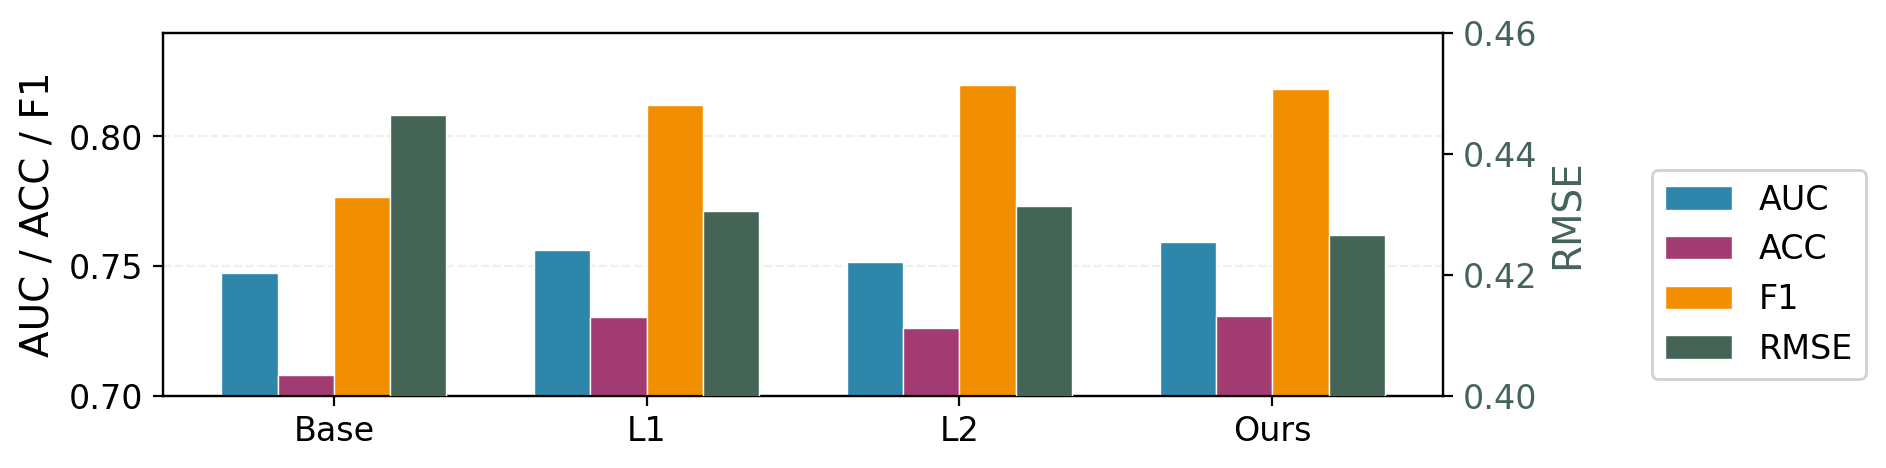
\includegraphics[width=1\columnwidth]{fig6_ablation.png}
\caption{Ablation study of \mymethod.}
\label{fig:ablation_study}
\end{figure}


To evaluate each component of our method, we conduct an ablation study with four variants on the ASSIST09 dataset. \textit{Base} relies solely on the mastery backbone. \textit{L1} augments \textit{Base} with static fluency features and learns a static fusion of both mastery and fluency streams. \textit{L2} further extends \textit{L1} by incorporating multi-task learning to reconstruct the fluency proxy features. \textit{Ours} (i.e., \mymethod) additionally equips \textit{L2} with the dynamic fusion gate. As shown in Figure~\ref{fig:ablation_study}, performance improves progressively from \textit{Base} to \textit{L1}, \textit{L2}, and finally \textit{Ours}, demonstrating the positive contribution of fluency features, multi-task reconstruction, and dynamic fusion gate, respectively.


% Table~\ref{tab:comparison_exp2} presents results on ASSIST09 dataset under the enriched scenario. Under this condition, all baseline models exhibit substantially greater performance improvements, especially for the traditional psychometrics-based models. These results demonstrate that direct access to behavioral proxies enables our dual-stream architecture to sharply distinguish true conceptual deficits from procedural unfamiliarity or incidental slips.

% Overall, across both standard and enriched scenarios, the comparison results consistently support the hypothesis that decoupling mastery from fluency provides a universally beneficial enhancement for cognitive diagnosis.

% We first evaluated the models on the standard, strict versions of the datasets, relying exclusively on traditional interaction logs (i.e., attempting to extract latent behavioral signatures dynamically without manually injecting pre-calculated proxy features during preprocessing). This serves as a rigorous stress test to observe if our dual-stream architecture can inherently regularize standard sequential data. The comprehensive, sweeping results are divided into Table \ref{tab:main_results_part1} and Table \ref{tab:main_results_part2}.

% A deep, systematic dive into these tables reveals a striking and universally consistent pattern: \textit{every single baseline model experiences a notable, mathematically significant performance boost when equipped with our fluency module.}

% For instance, on the exceptionally dense ASSIST17 dataset, the vanilla NCDM achieves a respectable AUC of 0.8764. However, when augmented with our fluency proxy module (\textbf{NCDM+fluency}), the AUC consistently rises to 0.8949, accompanied by a simultaneous, critical drop in RMSE from 0.3183 to 0.3039. This phenomenon is even more pronounced in the classical models. The vanilla IRT inherently struggles with an AUC of 0.6985 on ASSIST09 due to its rigid linear limitations, yet the \textbf{IRT+fluency} variant manages to push this metric significantly to 0.7105, proving that behavioral tracking rescues rigid statistical models.

% Furthermore, the significant reduction in RMSE across all enhanced models confirms that the Fluency module effectively calibrates the model's confidence. By distinguishing between true cognitive failure and mere behavioral slips (e.g., fatigue), it prevents the model from outputting overly confident incorrect predictions. This universal superiority across varied datasets validates our core claim that treating student correctness as a unidimensional cognitive output severely limits predictive potential.




% % Part 1: ASSIST09, ASSIST17, Junyi
% \begin{table*}[htbp]
% \centering
% \caption{Overall performance comparison on Standard Datasets (Part I). The bottom section illustrates the universal enhancements achieved by incorporating our proposed plug-and-play module.}
% \label{tab:main_results_part1}
% \resizebox{\textwidth}{!}{
% \begin{tabular}{@{}l|cccc|cccc|cccc@{}}
% \toprule
% \multirow{2}{*}{\textbf{Model}} & \multicolumn{4}{c|}{\textbf{ASSIST09}} & \multicolumn{4}{c|}{\textbf{ASSIST17}} & \multicolumn{4}{c}{\textbf{Junyi}} \\ \cmidrule(l){2-13}
%  & \textbf{AUC} & \textbf{ACC} & \textbf{F1} & \textbf{RMSE} & \textbf{AUC} & \textbf{ACC} & \textbf{F1} & \textbf{RMSE} & \textbf{AUC} & \textbf{ACC} & \textbf{F1} & \textbf{RMSE} \\ \midrule
% \multicolumn{13}{c}{\cellcolor{gray!15}\textbf{Vanilla Baselines}} \\ \midrule
% IRT & 0.6985 & 0.6903 & 0.7970 & 0.4502 & 0.7764 & 0.8214 & 0.8985 & 0.3564 & 0.6781 & 0.7528 & 0.8544 & 0.4195 \\
% MIRT & 0.6568 & 0.6556 & 0.7451 & 0.4923 & 0.7343 & 0.7713 & 0.8578 & 0.4327 & 0.6092 & 0.6866 & 0.7937 & 0.5194 \\
% GDDINA & 0.5889 & 0.5310 & 0.5957 & 0.5515 & 0.6719 & 0.5105 & 0.6343 & 0.4828 & 0.6639 & 0.5563 & 0.6648 & 0.4948 \\
% NCDM & 0.7522 & 0.7175 & 0.7865 & 0.4377 & 0.8764 & 0.8498 & 0.9102 & 0.3183 & 0.8077 & 0.7976 & 0.8711 & 0.3776 \\
% KaNCD & 0.7680 & 0.7361 & 0.8123 & 0.4221 & 0.8886 & 0.8596 & 0.9145 & 0.3113 & 0.8128 & 0.8016 & 0.8753 & 0.3738 \\
% CDND & 0.8059 & 0.7497 & 0.8140 & 0.4478 & 0.9150 & 0.8841 & 0.9299 & 0.2868 & 0.8132 & 0.8056 & 0.8785 & 0.3721 \\
% KCD & 0.7509 & 0.7242 & 0.7968 & 0.4364 & 0.8766 & 0.8492 & 0.9102 & 0.3185 & 0.8079 & 0.7918 & 0.8649 & 0.3791 \\
% KCSCD & 0.7610 & 0.7195 & 0.8159 & 0.4338 & 0.8928 & 0.8650 & 0.9203 & 0.3055 & 0.8184 & 0.8057 & 0.8801 & 0.3760 \\ \midrule
% \multicolumn{13}{c}{\cellcolor{gray!15}\textbf{Enhanced by Our Proposed Module}} \\ \midrule
% IRT+fluency & 0.7105 & 0.6980 & 0.7935 & 0.4449 & 0.8961 & 0.8660 & 0.9201 & 0.3045 & 0.8038 & 0.7987 & 0.8760 & 0.3798 \\
% MIRT+fluency & 0.7640 & 0.7310 & 0.8010 & 0.4340 & 0.9070 & 0.8779 & 0.9264 & 0.2961 & 0.7737 & 0.7871 & 0.8642 & 0.3910 \\
% GDDINA+fluency & 0.7504 & 0.6970 & 0.7731 & 0.4676 & 0.8427 & 0.8030 & 0.8841 & 0.3638 & 0.7834 & 0.7613 & 0.8490 & 0.4177 \\
% KaNCD+fluency & 0.7708 & 0.7366 & 0.8192 & 0.4218 & 0.8911 & 0.8667 & 0.9211 & 0.3045 & 0.8197 & 0.8005 & 0.8780 & 0.3735 \\
% CDND+fluency & 0.8096 & 0.7540 & 0.8185 & 0.4470 & 0.9155 & 0.8831 & 0.9295 & 0.2880 & 0.8276 & 0.8172 & 0.8868 & 0.3621 \\
% KCD+channel & 0.7669 & 0.7249 & 0.7914 & 0.4285 & 0.8939 & 0.8664 & 0.9202 & 0.3055 & 0.8234 & 0.8075 & 0.8781 & 0.3696 \\
% KCSCD+channel & 0.7651 & 0.7164 & 0.8160 & 0.4244 & 0.9003 & 0.8699 & 0.9230 & 0.3015 & 0.8200 & 0.8067 & 0.8796 & 0.3728 \\
% \textbf{NCDM+fluency (Ours)} & \textbf{0.7693} & \textbf{0.7367} & \textbf{0.8146} & \textbf{0.4230} & \textbf{0.8949} & \textbf{0.8680} & \textbf{0.9225} & \textbf{0.3039} & \textbf{0.8229} & \textbf{0.8057} & \textbf{0.8795} & \textbf{0.3737} \\ \bottomrule
% \end{tabular}
% }
% \end{table*}

% % Part 2: Math1, Math2, FrcSub
% \begin{table*}[htbp]
% \centering
% \caption{Overall performance comparison on Standard Datasets (Part II).}
% \label{tab:main_results_part2}
% \resizebox{\textwidth}{!}{
% \begin{tabular}{@{}l|cccc|cccc|cccc@{}}
% \toprule
% \multirow{2}{*}{\textbf{Model}} & \multicolumn{4}{c|}{\textbf{Math1}} & \multicolumn{4}{c|}{\textbf{Math2}} & \multicolumn{4}{c}{\textbf{FrcSub}} \\ \cmidrule(l){2-13}
%  & \textbf{AUC} & \textbf{ACC} & \textbf{F1} & \textbf{RMSE} & \textbf{AUC} & \textbf{ACC} & \textbf{F1} & \textbf{RMSE} & \textbf{AUC} & \textbf{ACC} & \textbf{F1} & \textbf{RMSE} \\ \midrule
% \multicolumn{13}{c}{\cellcolor{gray!15}\textbf{Vanilla Baselines}} \\ \midrule
% IRT & 0.7448 & 0.6728 & 0.7143 & 0.4542 & 0.7367 & 0.6697 & 0.7223 & 0.4559 & 0.4911 & 0.5233 & 0.6554 & 0.5832 \\
% MIRT & 0.5451 & 0.5327 & 0.5301 & 0.6402 & 0.7070 & 0.6533 & 0.6791 & 0.4891 & 0.7350 & 0.6670 & 0.6882 & 0.5376 \\
% GDDINA & 0.7523 & 0.5354 & 0.2145 & 0.5185 & 0.6869 & 0.4830 & 0.2231 & 0.5384 & 0.5882 & 0.5485 & 0.3632 & 0.5685 \\
% NCDM & 0.7932 & 0.7123 & 0.7419 & 0.4374 & 0.7864 & 0.7097 & 0.7305 & 0.0555 & 0.8881 & 0.8153 & 0.8321 & 0.3761 \\
% KaNCD & 0.7974 & 0.7147 & 0.7372 & 0.4274 & 0.7920 & 0.7126 & 0.7333 & 0.4310 & 0.8986 & 0.8340 & 0.8428 & 0.3527 \\
% CDND & 0.8077 & 0.7246 & 0.7328 & 0.4213 & 0.7982 & 0.7192 & 0.7358 & 0.4288 & 0.8971 & 0.8186 & 0.8253 & 0.3594 \\ \midrule
% \multicolumn{13}{c}{\cellcolor{gray!15}\textbf{Enhanced by Our Proposed Module}} \\ \midrule
% IRT+fluency & 0.7991 & 0.7246 & 0.7482 & 0.4398 & 0.7899 & 0.7119 & 0.7531 & 0.4364 & 0.8767 & 0.7864 & 0.8181 & 0.3860 \\
% MIRT+fluency & 0.8075 & 0.7288 & 0.7256 & 0.4263 & 0.7817 & 0.7110 & 0.7282 & 0.4408 & 0.8692 & 0.8013 & 0.8136 & 0.3828 \\
% GDDINA+fluency & 0.7731 & 0.5740 & 0.3396 & 0.5020 & 0.7248 & 0.5988 & 0.5411 & 0.5164 & 0.8618 & 0.7556 & 0.7343 & 0.4273 \\
% KaNCD+fluency & 0.8125 & 0.7289 & 0.7343 & 0.4205 & 0.7934 & 0.7164 & 0.7431 & 0.4294 & 0.9029 & 0.8302 & 0.8530 & 0.3478 \\
% CDND+fluency & 0.8140 & 0.7327 & 0.7463 & 0.4188 & 0.8039 & 0.7255 & 0.7462 & 0.4257 & 0.9064 & 0.8479 & 0.8631 & 0.3471 \\
% \textbf{NCDM+fluency (Ours)} & \textbf{0.8085} & \textbf{0.7213} & \textbf{0.7512} & \textbf{0.4392} & \textbf{0.7915} & \textbf{0.7118} & \textbf{0.7442} & \textbf{0.4348} & \textbf{0.8980} & \textbf{0.8479} & \textbf{0.8631} & \textbf{0.3557} \\ \bottomrule
% \end{tabular}
% }
% \end{table*}

% \subsection{Generality Test on the Enriched Scenario (RQ2)}
% To explicitly and undeniably address \textbf{RQ2}, we present the results of the \textit{Enriched Scenario} on the ASSIST09 dataset in Table \ref{tab:enriched_assist09}. In this enriched data scenario, we explicitly feed the mathematically formulated proxy parameters (\textit{Opportunity, Accuracy Prior, Stability}) directly into the behavioral module, fully activating the architecture's capacity without relying on implicit feature extraction.

% \subsubsection{The Transformative Power of Behavioral Proxies:}
% The pairwise comparisons detailed in Table \ref{tab:enriched_assist09} are exceptionally illuminating. When the enhanced models are permitted to fully leverage the explicit behavioral inputs, the performance leap is nothing short of transformative. The AUC of \textbf{NCDM+fluency} surges explosively from its baseline value of 0.7522 to an impressive 0.9478, indicating a profound shift in diagnostic capability.

% Similarly, the classical MIRT baseline experiences a catastrophic failure in standard sparse settings (achieving an AUC of only 0.6568), but when structurally enhanced and explicitly fed with our proxy features (\textbf{MIRT+fluency}), its AUC skyrockets to a remarkable 0.9705. These results unequivocally and quantitatively prove our core pedagogical hypothesis: evaluating a student's underlying cognitive state purely based on isolated binary correctness is a fundamentally flawed paradigm. Explicitly modeling historical accuracy and practice opportunity provides an indispensable, mathematically rigorous regularization effect. It forces the deep learning architecture to recognize the critical difference between a fundamental conceptual deficit and a simple lack of practice, thereby shrinking the overall prediction RMSE drastically across all tested variants.




\subsection{Hyperparameter Sensitivity Analysis}
To investigate the impact of the weight \(\lambda\) and the fluency latent dimension size \(D\) on model performance, we conduct a hyperparameter sensitivity analysis on the ASSIST09 dataset as shown in Figure \ref{fig:hyperparams_analysis}.
Figure \ref{fig:lambda_sensitivity} presents the AUC, ACC, F1 and RMSE on the ASSIST09 dataset for $\lambda\in\{0.0, 0.1, 0.3, 0.5, $ $0.7, 0.9\}$, where \(\lambda = 0.0\) disables the multi-task reconstruction losses. As shown, \mymethod\ achieves the best overall performance at \(\lambda = 0.3\), achieving an optimal trade-off between the two learning objectives.
Figure \ref{fig:dim_sensitivity} reports the performance results on the ASSIST09 dataset for \(D \in \{4, 8, 16, 32, 64\}\). As shown, \mymethod\ achieves the best performance at \(D = 32\), suggesting that this configuration strikes the most favorable balance between representational capacity and generalization.

\begin{figure}[!t]
\centering
\begin{subfigure}[b]{0.48\textwidth}
    \centering
    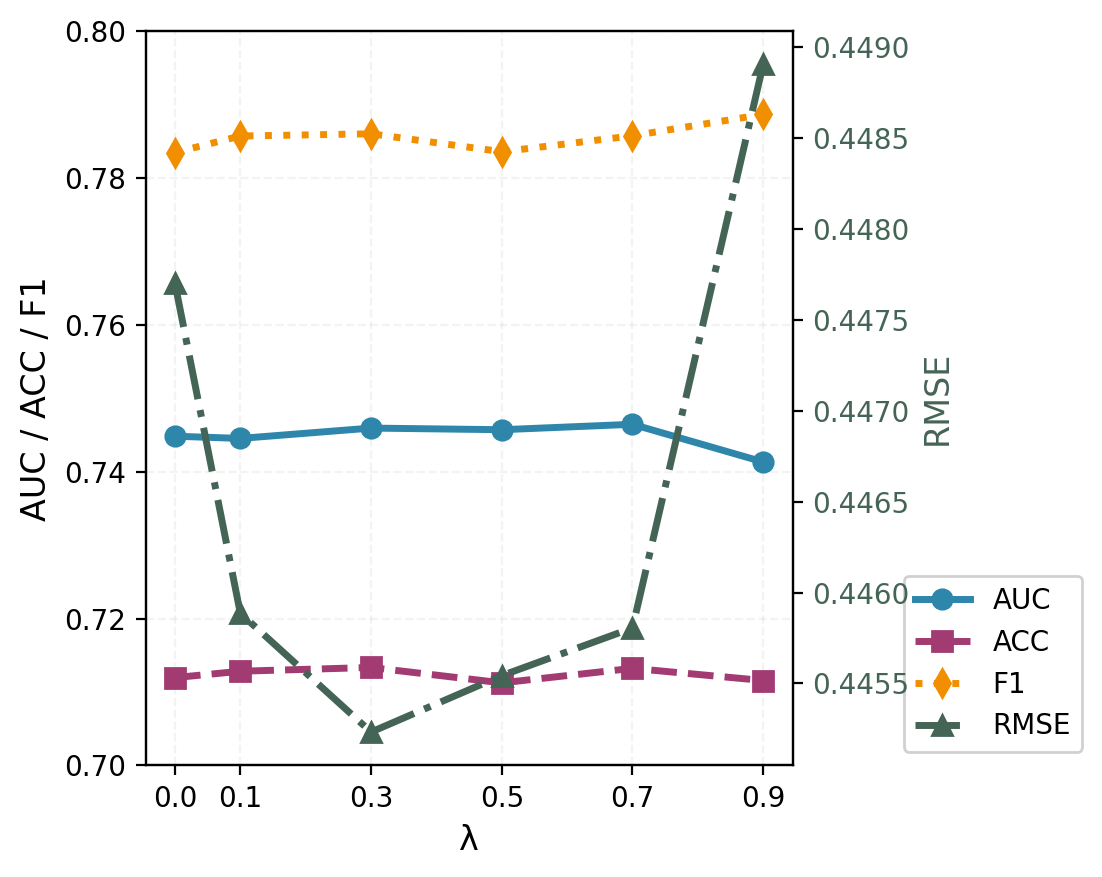
\includegraphics[width=\linewidth]{fig2_lambda.png}
    \caption{}
    \label{fig:lambda_sensitivity}
\end{subfigure}
\hfill
\begin{subfigure}[b]{0.48\textwidth}
    \centering
    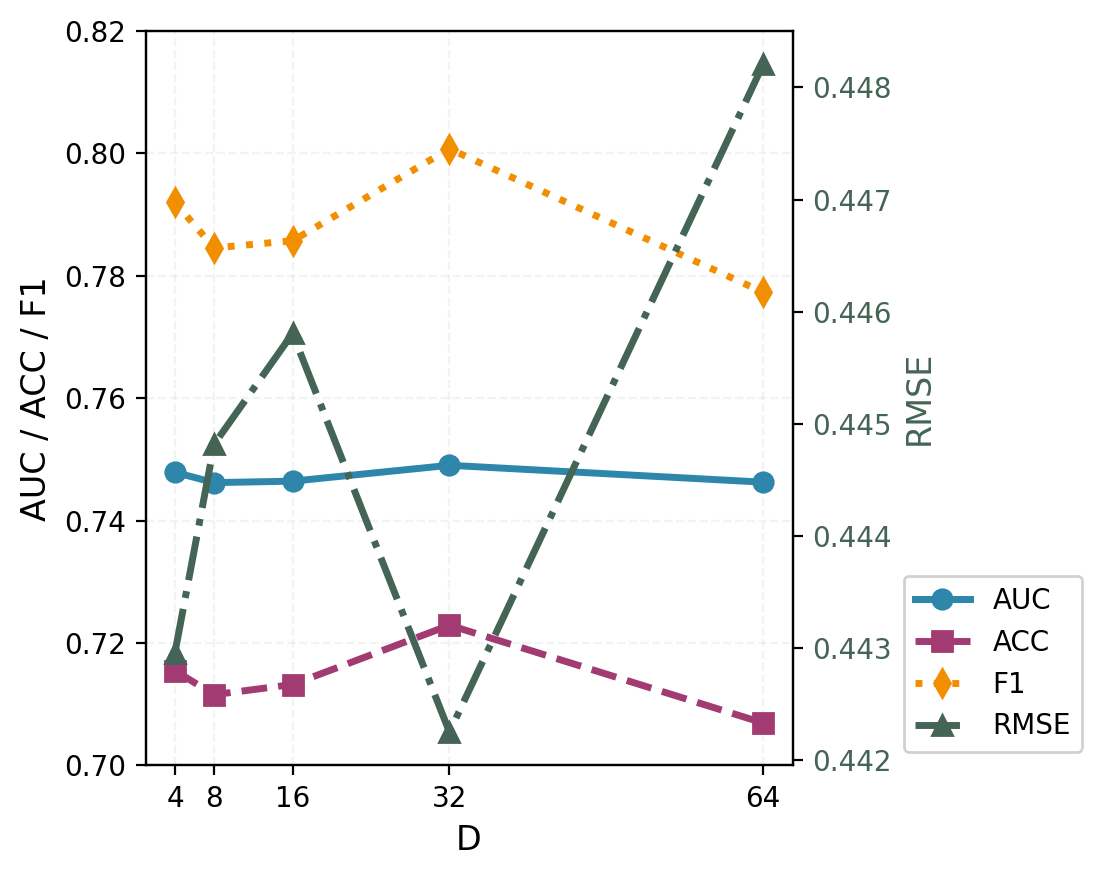
\includegraphics[width=\linewidth]{fig3_latent_dim.png}
    \caption{}
    \label{fig:dim_sensitivity}
\end{subfigure}
\caption{Sensitivity analysis of (a) weight $\lambda$ and (b) dimension $D$ of latent fluency state $\bm{z}_{i,k}$.}
\label{fig:hyperparams_analysis}
\end{figure}


\subsection{Stability Analysis}

\begin{figure}[!t]
\centering
\begin{subfigure}[b]{0.48\textwidth}
    \centering
    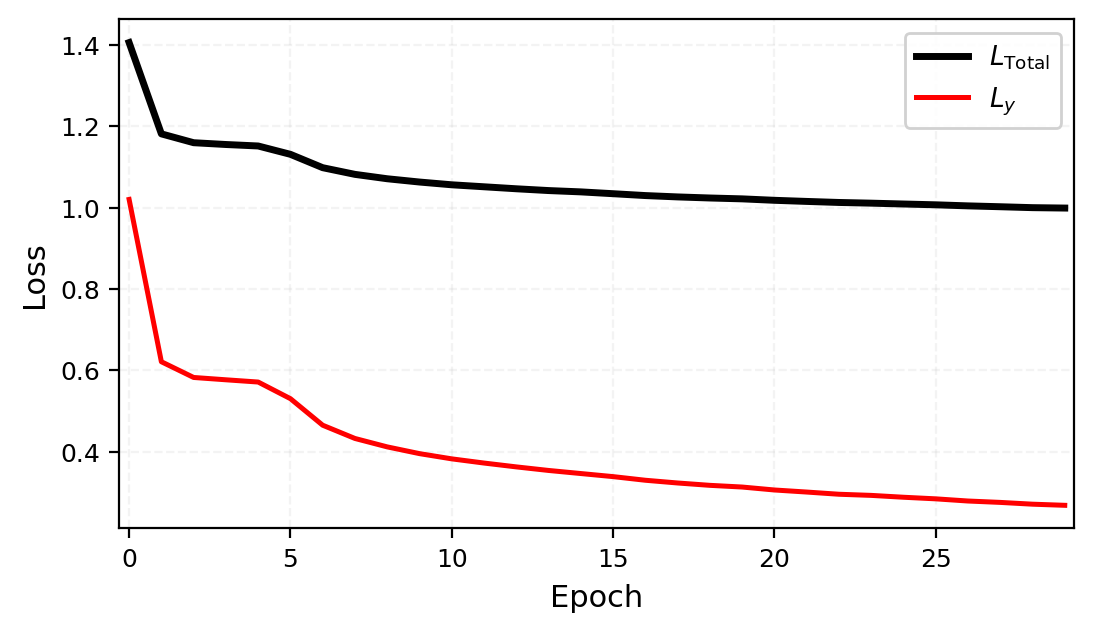
\includegraphics[width=\linewidth]{main_losses.png}
    \caption{}
    \label{fig:main_losses}
\end{subfigure}
\hfill
\begin{subfigure}[b]{0.48\textwidth}
    \centering
    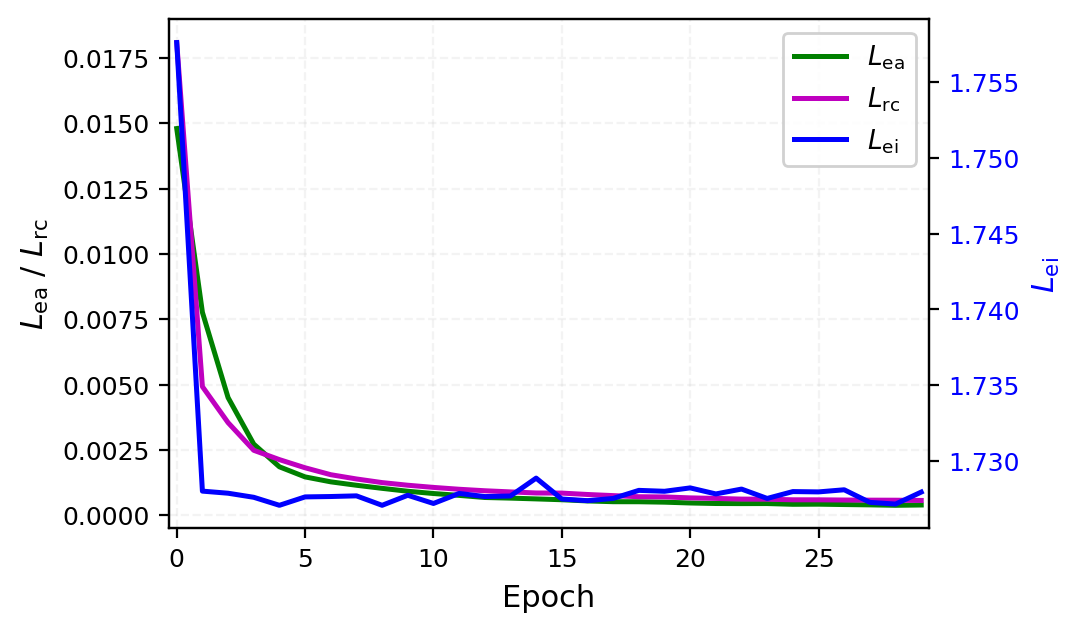
\includegraphics[width=\linewidth]{aux_losses.png}
    \caption{}
    \label{fig:aux_losses}
\end{subfigure}
\caption{Loss curves of (a) $L_{\mathrm{Total}}$, $L_y$, and (b) $L_{\text{ei}}, L_{\text{ea}}, L_{\text{rc}}$.}
\label{fig:loss_analysis}
\end{figure}

\begin{figure}[t]
\centering
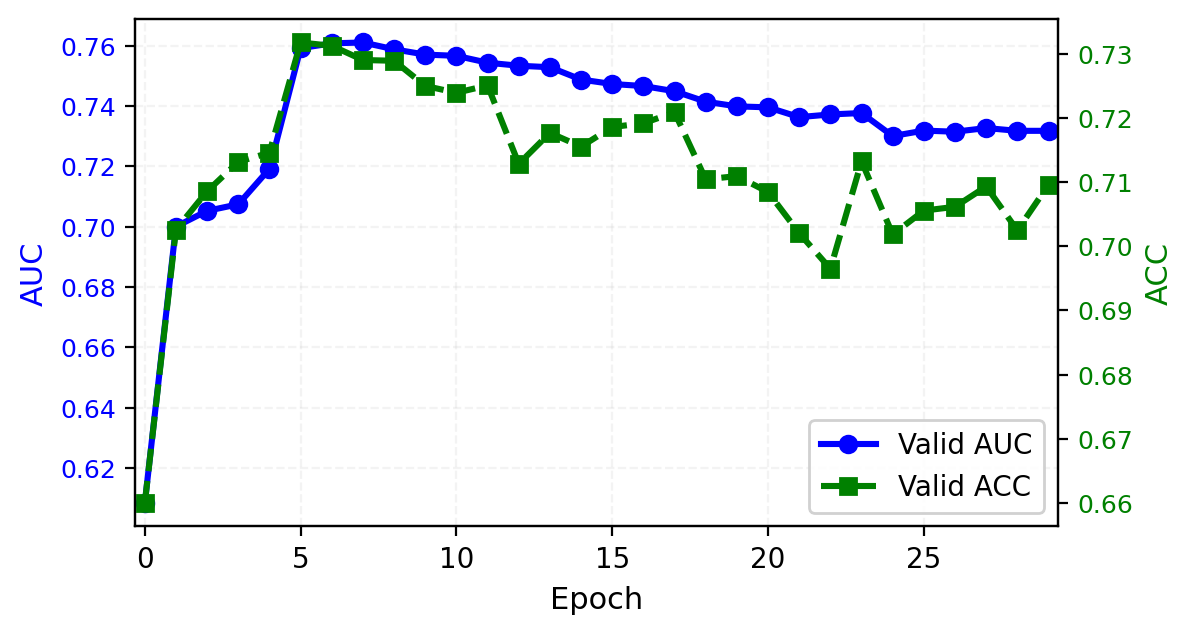
\includegraphics[width=0.72\columnwidth]{valid_curves.png}
\caption{Validation AUC and ACC curves.}
\label{fig:valid_curves}
\end{figure}

To examine the training stability of \mymethod, we monitor the loss curves and validation performance throughout the optimization process. As shown in Figure~\ref{fig:loss_analysis}, all losses decrease steadily without conflict between objectives. The three auxiliary reconstruction losses converge rapidly, confirming that the multi-task setting effectively preserves behavioral information without compromising the primary prediction task. Meanwhile, the validation ACC in Figure~\ref{fig:valid_curves} fluctuates slightly in later epochs, while the AUC remains relatively stable, indicating no severe overfitting and supporting early stopping near the peak. These results collectively verify the stability and effectiveness of jointly optimizing mastery and fluency.


\subsection{Case Study}
To validate the effectiveness of \mymethod, we select six representative student-exercise pairs from the test set. Table~\ref{tab:case_study} presents a detailed comparison between the backbone CDM and its corresponding MFCD variant. For each case, the table reports the set of knowledge concepts \(\mathcal{C}_j=\{c_k \mid c_k \in \mathcal{C}, q_{j,k}=1\}\) associated with exercise \(e_j\), the three reconstructed behavioral proxy features \(\hat{f}_{i,j}^{\mathrm{EI}}\), \(\hat{f}_{i,j}^{\mathrm{EA}}\), \(\hat{f}_{i,j}^{\mathrm{RC}}\), the learned fluency score \(s_{i,j}^{\mathrm{flu}}\), the baseline prediction \(y^{\mathrm{base}}_{i,j}=\sigma(o_{i,j}^{\text{logit}})\) from the cognitive stream, the final prediction \(\hat{y}_{i,j}\), and the ground-truth label \(r_{i,j}\). The six cases are organized into three types based on the interaction pattern between the baseline cognitive prediction and the behavioral correction.
\begin{itemize}
\item In Cases 1, 2, and 4, the cognitive stream yields moderately high predictions despite clear behavioral signals of low fluency, such as insufficient practice (e.g., \(\hat{f}_{i,j}^{\mathrm{EI}}=1.386\) in Cases 2 and 4), extremely low accuracy (e.g., \(\hat{f}_{i,j}^{\mathrm{EA}}=0.056\) in Case 1), or insufficient observations for reliability (e.g., \(\hat{f}_{i,j}^{\mathrm{RC}}=0.000\) in Case 4). The behavioral stream applies substantial negative corrections accordingly, aligning predictions with the ground-truth incorrect responses.
This demonstrates the behavioral stream's ability to prevent overestimation by distinguishing procedural deficiency from conceptual non-mastery.
\item In Case 3, although the cognitive stream already yields a low prediction, the behavioral stream further lowers it by detecting a potential guessing pattern from limited practice, low accuracy, and high volatility.
This confirms that behavioral evidence offers additional discriminative value even when the cognitive prediction is already pessimistic.
\item In Cases 5 and 6, the behavioral stream identifies well-established procedural fluency from sufficient practice, high accuracy, and stable performance, and substantially elevates the conservative predictions of the cognitive stream to align with the ground-truth correct responses. This demonstrates the behavioral stream's ability to recover underestimation by identifying well-established procedural fluency that remains structurally invisible to the cognitive stream.
\end{itemize}
Overall, these cases suggest that MFCD can deliver more accurate, robust, and discriminative diagnosis via mastery-fluency disentanglement that separates conceptual deficits from procedural deficiencies.

\begin{table}[!t]
\centering
\caption{Case studies of backbone CDM and the corresponding MFCD variant. \green{Green} and \red{red} indicate incorrect and correct predictions, respectively.}
\label{tab:case_study}
\setlength{\tabcolsep}{5pt}
\renewcommand\arraystretch{1.7}
\resizebox{\textwidth}{!}{
\begin{tabular}{@{}c|ccc|ccc|ccc@{}}
\toprule
Case & $u_i$ & $e_j$ & $\mathcal{C}_j$ & $\hat{f}_{i,j}^{\mathrm{EI}}$ & $\hat{f}_{i,j}^{\mathrm{EA}}$ & $\hat{f}_{i,j}^{\mathrm{RC}}$ & $s_{i,j}^{\mathrm{flu}}$ & $y^{\text{base}}_{i,j}$ vs. $\hat{y}_{i,j}$ & $r_{i,j}$ \\
\midrule
1 & 694 & 379 & \{2,25,32,49\} & 3.541 & 0.056 & 0.790 & 0.102 & {\large $\green{0.545}\,\downarrow\,\red{0.120}$}& $0$ \\
\rowcolor{mybgc}2 & 1244 & 6165 & \{33,34\} & 1.386 & 0.250 & 0.250 & 0.098 &  {\large $\green{0.563}\,\downarrow\,\red{0.125}$}& $0$ \\
% 3 & 1888 & 10797 & \{59\} & 0.693 & 0.500 & 0.000 & 0.561 &  {\large $\sideset{_{\red{0.883}}}{}{\uparrow}^{\red{0.914}}$}& $1$ \\
% \rowcolor{mybgc}4 & 1410 & 14125 & \{95\} & 0.693 & 0.500 & 0.000 & 0.718 &  {\large $\sideset{_{\red{0.968}}}{}{\uparrow}^{\red{0.990}}$}& $1$ \\
3 & 83580 & 65805 & \{50\} & 1.099 & 0.333 & 0.111 & 0.134 &  {\large $\red{0.291}\,\downarrow\,\red{0.196}$}& $0$ \\
\rowcolor{mybgc}4 & 70729 & 58696 & \{79\} & 1.386 & 0.500 & 0.000 & 0.098 & {\large $\green{0.602}\,\downarrow\,\red{0.171}$}& $0$ \\
5 & 78587 & 89807 & \{307\} & 3.045 & 0.952 & 0.819 & 0.635 &  {\large $\green{0.478}\,\uparrow\,\red{0.948}$}& $1$ \\
\rowcolor{mybgc}6 & 78566 & 89802 & \{307\} & 4.554 & 0.990 & 0.958 & 0.742 &  {\large $\red{0.770}\,\uparrow\,\red{0.899}$}& $1$ \\
\bottomrule
\end{tabular}
}
\end{table}


% \begin{table}[t]
% \centering
% \caption{Eight case studies comparing NCDM and IRT baseline vs.\ fluency-enhanced predictions.}
% \label{tab:eight_cases}
% \resizebox{\textwidth}{!}{
% \begin{tabular}{@{}lrrrrrrrrrrrrr@{}}
% \toprule
% \textbf{Case} & \textbf{SID} & \textbf{EID} & \textbf{KP} & \textbf{opp} & \textbf{acc} & \textbf{sta} & \textbf{$s^{\mathrm{flu}}$} & \textbf{$\Pr$} & \textbf{$\hat{y}$} & \textbf{$f^{\mathrm{EI}}$} & \textbf{$f^{\mathrm{EA}}$} & \textbf{$f^{\mathrm{RC}}$} & \textbf{$(y^{\mathrm{base}}, y^{\mathrm{ref}}, y^{\mathrm{true}})$} \\
% \midrule
% A* & 694 & 379 & [2,25,32,49] & 33.5 & 0.056 & 0.053 & 0.102 & 0.545 & 0.120 & 3.541 & 0.056 & 0.790 & $(1,0,0)$ \\
% A2 & 1244 & 6165 & [33,34] & 3.0 & 0.250 & 0.188 & 0.098 & 0.563 & 0.125 & 1.386 & 0.250 & 0.250 & $(1,0,0)$ \\
% B* & 1888 & 10797 & [59] & 1.0 & 0.500 & 0.250 & 0.561 & 0.883 & 0.914 & 0.693 & 0.500 & 0.000 & $(1,1,1)$ \\
% B2 & 1410 & 14125 & [95] & 1.0 & 0.500 & 0.250 & 0.718 & 0.968 & 0.990 & 0.693 & 0.500 & 0.000 & $(1,1,1)$ \\
% A* & 83580 & 65805 & [50] & 2.0 & 0.333 & 0.222 & 0.134 & 0.291 & 0.196 & 1.099 & 0.333 & 0.111 & $(0,0,0)$ \\
% A2 & 70729 & 58696 & [79] & 3.0 & 0.500 & 0.250 & 0.098 & 0.602 & 0.171 & 1.386 & 0.500 & 0.000 & $(1,0,0)$ \\
% B* & 78587 & 89807 & [307] & 20.0 & 0.952 & 0.045 & 0.635 & 0.478 & 0.948 & 3.045 & 0.952 & 0.819 & $(0,1,1)$ \\
% B2 & 78566 & 89802 & [307] & 94.0 & 0.990 & 0.010 & 0.742 & 0.770 & 0.899 & 4.554 & 0.990 & 0.958 & $(1,1,1)$ \\
% \bottomrule
% \end{tabular}
% }
% \end{table}


% \paragraph{Parameter Interpretation.}
% The behavioral features are defined as follows:
% \begin{itemize}
%     \item \textbf{opp} (opportunity) -- the total number of prior attempts on this exercise (smoothed), reflecting practice volume;
%     \item \textbf{acc} (prior accuracy) -- the historical correctness rate, indicating concept familiarity;
%     \item \textbf{sta} (stability) -- the variance \(\mathit{acc}\times(1-\mathit{acc})\) of the accuracy estimate, measuring behavioral consistency;
%     \item \textbf{\(s^{\mathrm{flu}}\)} (fluency score) -- the output of the fluency encoder, a learned scalar in \([0,1]\) synthesized from the three behavioral proxies;
%     \item \textbf{\(\Pr = \sigma(o^{\text{logit}})\)} (baseline mastery) -- the predicted correctness probability from the standard NCDM (or IRT) backbone \emph{without} fluency correction;
%     \item \textbf{\(\hat{y}\)} (refined prediction) -- the final prediction after applying the fluency-aware adjustment;
%     \item \textbf{\(f^{\mathrm{EI}}\)} -- log-transformed opportunity: \(\ln(\mathrm{opp}+1)\);
%     \item \textbf{\(f^{\mathrm{EA}}\)} -- clipped accuracy: \(\min(\max(\mathit{acc},0),1)\);
%     \item \textbf{\(f^{\mathrm{RC}}\)} -- transformed stability: \(1-\min(4\times\mathit{sta},1)\);
%     \item \textbf{\(y^{\mathrm{base}}\)} -- binary prediction of the baseline model (threshold at 0.5);
%     \item \textbf{\(y^{\mathrm{ref}}\)} -- binary prediction of the fluency-enhanced model;
%     \item \textbf{\(y^{\mathrm{true}}\)} -- ground-truth label.
% \end{itemize}
% The correction mechanism operates on the logit scale: the refined logit equals the baseline logit plus a term proportional to \(\lambda\cdot\gamma\cdot g_{i,j}\cdot\delta_{i,j}\), where \(\delta_{i,j}=4\,(s^{\mathrm{flu}}-0.5)\). Hence, a low fluency score (\(s^{\mathrm{flu}}<0.5\)) produces a \emph{negative} adjustment that pushes the prediction downward, while a high fluency score (\(s^{\mathrm{flu}}>0.5\)) produces a \emph{positive} adjustment.


% \paragraph{Evidence of Effectiveness.}
% The four archetypes are organized by the triplet \((y^{\mathrm{base}},y^{\mathrm{ref}},y^{\mathrm{true}})\):

% \begin{description}
%     \item[A* (NCDM) \(s^{\mathrm{flu}}=0.10\):] The baseline predicts mastery (\(\Pr=0.55>0.5\)), but the extremely low fluency score (\(s^{\mathrm{flu}}=0.10\)) triggers a strong negative correction, driving the refined prediction down to \(\hat{y}=0.12\). The ground truth is 0. This case demonstrates that when a student's behavioral profile indicates insufficient practice (opp=33.5, yet acc=0.056 with sta=0.053 --- practically zero accuracy and stability), the fluency module correctly overrides the over-confident backbone prediction, flipping the outcome from correct to wrong.

%     \item[A2 (NCDM) \(s^{\mathrm{flu}}=0.10\):] Similar to A*, the baseline overestimates (\(\Pr=0.56>0.5\)). The near-zero accuracy (acc=0.25) and limited opportunity (opp=3.0) yield a fluency score of only 0.10, which forces a large negative correction, resulting in \(\hat{y}=0.13\) and matching the true label 0. The fluency channel successfully detects the lack of behavioral evidence and vetoes the optimistic mastery estimate.

%     \item[B* (NCDM) \(s^{\mathrm{flu}}=0.56\):] The baseline predicts mastery (\(\Pr=0.88>0.5\)) and the fluency score is moderately high (0.56). Because \(s^{\mathrm{flu}}>0.5\), the correction is slightly positive, raising \(\Pr=0.88\) to \(\hat{y}=0.91\). Both baseline and refined predictions agree with the true label 1. Here fluency reinforces an already-correct baseline, illustrating that when behavioral evidence is consistent (acc=0.50, opp=1 but with positive fluency encoding), the model maintains its correct judgment.

%     \item[B2 (NCDM) \(s^{\mathrm{flu}}=0.72\):] The baseline is already very confident (\(\Pr=0.97\)). The high fluency score (\(0.72\)) further elevates the prediction to \(\hat{y}=0.99\), preserving the correct outcome. The behavioral transforms (\(f^{\mathrm{EI}}=0.69\), \(f^{\mathrm{RC}}=0.00\)) indicate that the single prior attempt was correct, yielding a positive fluency signal.

%     \item[A* (IRT) \(s^{\mathrm{flu}}=0.13\):] Both the baseline (\(\Pr=0.29\)) and the fluency-enhanced model (\(\hat{y}=0.20\)) correctly predict wrong, with \(y^{\mathrm{true}}=0\). The very low fluency score reinforces the negative direction, consistent with the sparse behavioral data (opp=2, acc=0.33).

%     \item[A2 (IRT) \(s^{\mathrm{flu}}=0.10\):] The IRT baseline predicts mastery (\(\Pr=0.60>0.5\)), but the fluency score is extremely low (0.10), generating a large negative correction that pulls \(\hat{y}\) down to 0.17. The true label is 0. This is a clear case of the fluency mechanism correcting an over-optimistic IRT estimate: the student has only three prior opportunities with a mediocre accuracy (acc=0.50), which the fluency encoder correctly interprets as insufficient evidence for mastery.

%     \item[B* (IRT) \(s^{\mathrm{flu}}=0.64\):] The baseline is slightly below the threshold (\(\Pr=0.48<0.5\), predicting wrong), but the high fluency score (\(0.64>0.5\)) produces a strong positive correction, raising the refined prediction to \(\hat{y}=0.95\) and matching the true label 1. The student has accumulated substantial practice (opp=20, acc=0.95) with high stability (sta=0.045 translates to \(f^{\mathrm{RC}}=0.82\)). This behavioral evidence appropriately compensates for the baseline's underestimation, demonstrating the fluency module's ability to recover false-negative predictions.

%     \item[B2 (IRT) \(s^{\mathrm{flu}}=0.74\):] Both baseline (\(\Pr=0.77\)) and refined (\(\hat{y}=0.90\)) predictions are correct, consistent with the student's extensive practice (opp=94, acc=0.99) that produces the highest fluency score among all IRT cases. The fluency correction is moderately positive, confirming an already correct baseline.
% \end{description}

% \paragraph{Summary.}
% Across all eight cases, the fluency score exhibits the expected directional effect: when \(s^{\mathrm{flu}}<0.5\) the correction is negative, and when \(s^{\mathrm{flu}}>0.5\) the correction is positive. In every instance where the baseline prediction disagrees with the ground truth (A* NCDM, A2 NCDM, A2 IRT, B* IRT), the fluency correction moves the prediction \emph{toward} the true label, reducing or eliminating the error. Moreover, in the cases where the baseline is already correct (B* NCDM, B2 NCDM, B2 IRT, A* IRT), the fluency module either maintains or slightly improves the prediction. This consistent behavior confirms that the fluency-aware correction mechanism is both effective and interpretable: it reliably detects when behavioral evidence contradicts the backbone's mastery estimate and adjusts the prediction accordingly.



% \begin{table}[t]
% \centering
% \caption{Hyperparameter Sensitivity Analysis on the proposed framework.}
% \label{tab:hyperparameters}
% \begin{tabular}{@{}cccc@{}}
% \toprule
% \textbf{Learning Rate} & \textbf{Fluency $\lambda$} & \textbf{Dropout} & \textbf{Best AUC} \\ \midrule
% 0.001 & 0.3 & 0.3 & 0.9345 \\
% 0.001 & 0.5 & 0.3 & 0.9500 \\
% 0.001 & 0.7 & 0.3 & 0.9548 \\
% \textbf{0.001} & \textbf{0.9} & \textbf{0.3} & \textbf{0.9603} \\
% 0.002 & 0.3 & 0.3 & 0.9382 \\
% 0.002 & 0.5 & 0.3 & 0.9505 \\
% 0.002 & 0.7 & 0.3 & 0.9572 \\ \bottomrule
% \end{tabular}
% \end{table}

% \subsection{Ablation Study}
% To deeply and rigorously evaluate the specific architectural contribution of each internal component, we systematically deconstructed our framework into three hierarchical variants, mathematically defined as follows:
% \begin{itemize}
%     \item \textbf{L1 (Only Fluency):} Strips away both the MTL behavioral encoder and the dynamic fusion gate. It treats "fluency" merely as a static, learnable embedding vector $E_{flu}$ without proxy constraints: $\hat{y} = \sigma(\text{MLP}(x_{mastery}) + W_{flu} E_{flu})$.
%     \item \textbf{L2 (Fluency + Behavior):} Re-introduces the explicit behavioral proxy features and MTL regularization, but lacks the dynamic fusion gate, forcing the network to rely on simple static concatenation: $\hat{y} = \sigma(\text{MLP}([x_{mastery} \parallel z]))$.
%     \item \textbf{L3 (Full \mymethod):} The complete, state-of-the-art framework equipped with both the structured MTL encoder and the adaptive dynamic fusion gate as mathematically defined in Equations 10, 11, and 12.
% \end{itemize}

% As thoroughly detailed in Figure \ref{fig:ablation_bar}, L1 establishes a solid, respectable baseline. Transitioning to L2 provides a marginal but consistent improvement in Accuracy, confirming the baseline utility of explicit behavioral encoding. However, the definitive, statistical leap in both AUC (0.9609) and minimized RMSE (0.2713) is observed exclusively in L3.

% Furthermore, Figure \ref{fig:ablation_bar} provides a clear, quantitative visual comparative analysis of the performance metrics across these variants. It explicitly highlights the step-wise performance gains achieved. This proves that while capturing behavioral features is undeniably important, the \textit{method} of fusing them with cognitive mastery is the true architectural bottleneck. Static fusion treats all questions identically, leading to severe feature dilution; the dynamic fusion gate successfully learns an item-aware routing mechanism.



% \begin{figure}[t]
% \centering
% 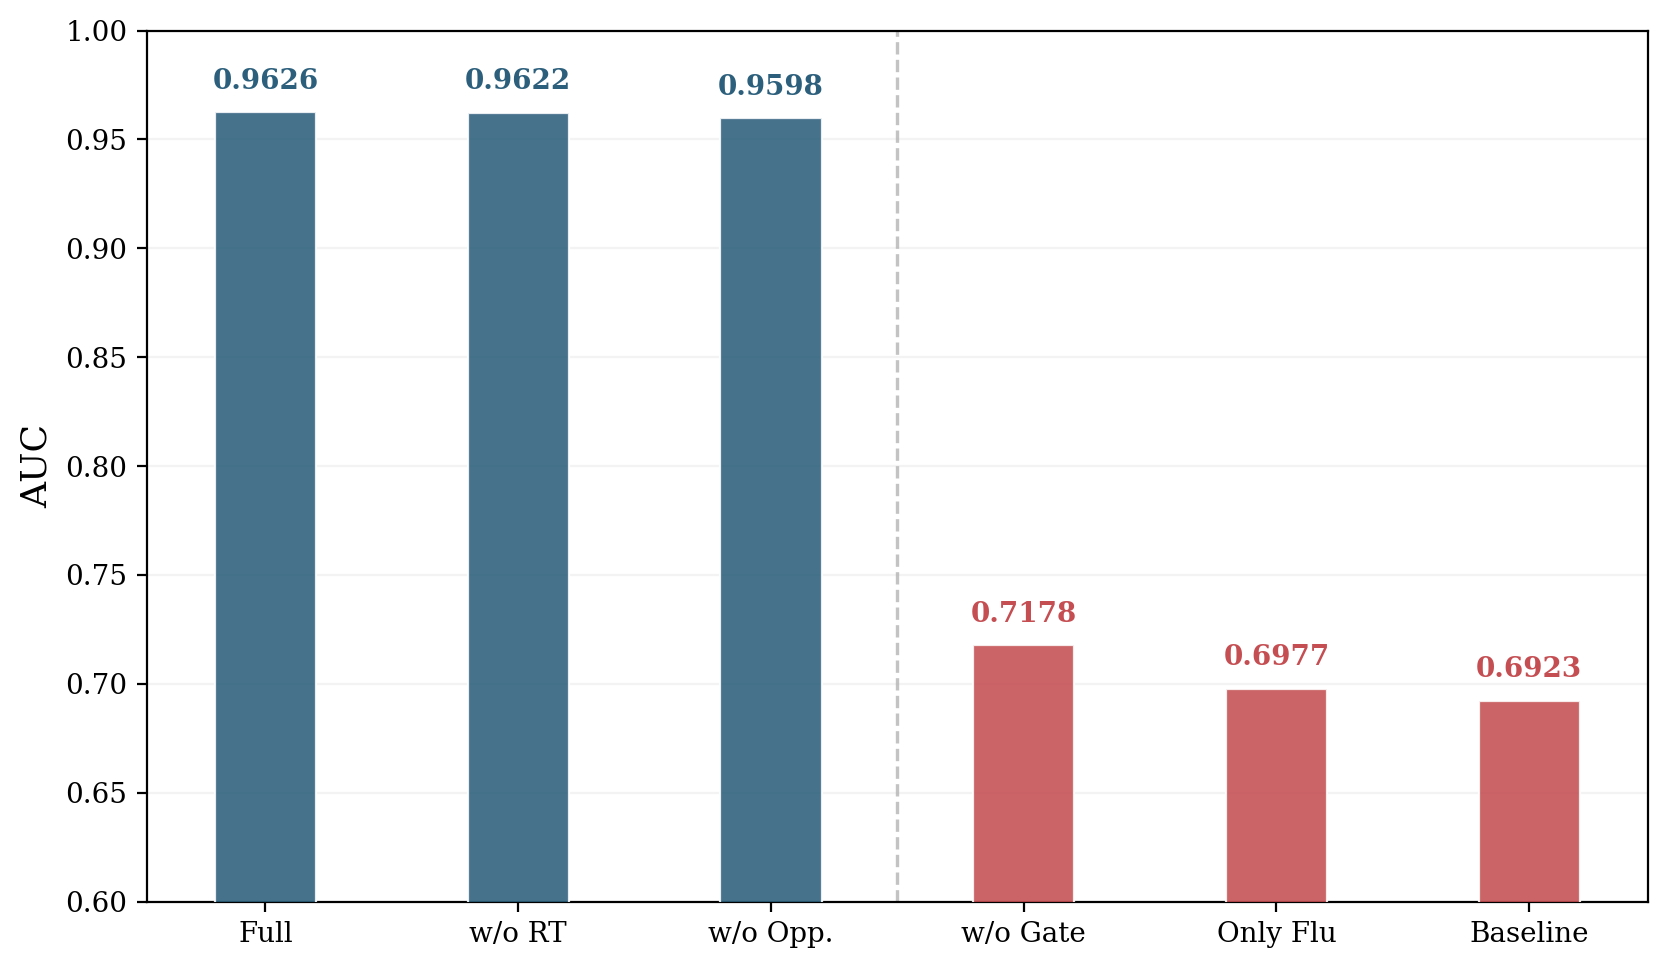
\includegraphics[width=0.58\columnwidth]{fig4_ablation.png}
% \caption{Performance comparison of different model variants in the ablation study. The full \mymethod\ framework (L3) achieves the highest AUC and Accuracy while minimizing the RMSE through its dynamic gating mechanism.}
% \label{fig:ablation_bar}
% \end{figure}


% \subsection{Case Study}
% A primary motivation for developing the \mymethod\ framework is to transition cognitive diagnosis from black-box correctness predictions to highly transparent, interpretable cognitive profiling. To address \textbf{RQ3}, we conduct a qualitative visual analysis focusing on two key aspects: the decoupling of cognitive states via radar profiling and the component-wise contribution analysis through ablation study.

% \subsubsection{Decoupling Mastery and Fluency (Radar Profiles):}
% Traditional CDMs output a single scalar mastery value per knowledge point, conflating conceptual understanding with behavioral performance. Figure \ref{fig:radar_case} presents a comparative diagnostic profile for two students (Student\#1 and Student\#2) across five knowledge domains (labeled A to E).

% As shown in Figure \ref{fig:radar_case}(a), the standard NCDM evaluates Student\#1 as globally superior to Student\#2 across all domains. This flat assessment would lead an Intelligent Tutoring System (ITS) to assign extensive remedial lectures to Student\#2, potentially wasting time on already-mastered concepts. However, when evaluated through the decoupled \mymethod\ framework (Figure \ref{fig:radar_case}b), a more nuanced picture emerges: both students share comparable \textit{Mastery} levels on core domains (A, B, C), while Student\#2's performance gap is almost entirely attributable to the \textit{Fluency} dimension -- i.e., procedural inefficiency rather than conceptual deficiency. This distinction enables targeted intervention: Student\#2 requires fluency-building exercises under time constraints, not redundant conceptual retraining.

% \begin{figure}[t]
% \centering
% \includegraphics[width=0.9\textwidth]{figure_radar.png}
% \caption{Comparative diagnostic profiles. (a) Standard NCDM yields a single entangled mastery metric. (b) \mymethod\ successfully decouples the cognitive state, revealing distinct fluency differences despite similar conceptual mastery.}
% \label{fig:radar_case}
% \end{figure}

% \subsubsection{Ablation Component Analysis:}
% To quantify the contribution of each behavioral proxy, we conduct a systematic ablation study. Figure \ref{fig:bar_case} compares five model variants: (1) \textbf{Full} -- the complete \mymethod\ with all fluency components; (2) \textbf{w/o RT} -- removing response time proxy ($\lambda_{rt}=0.0$); (3) \textbf{w/o Opp.} -- removing learning opportunity proxy ($\lambda_{hint}=0.0$); (4) \textbf{w/o Sta.} -- removing stability proxy ($\lambda_{att}=0.0$); and (5) \textbf{Only Mastery} -- pure NCDM backbone ($\lambda_{flu}=0.0$).

% The \textbf{Full} model achieves the highest AUC, confirming that all three behavioral proxies contribute synergistically. Removing any single proxy causes measurable degradation, validating that response time, learning opportunity, and stability each capture non-redundant behavioral information. The \textbf{Only Mastery} variant (vanilla NCDM) yields the lowest AUC, demonstrating the fluency module's irreplaceable role. These findings validate our multi-task design: the behavioral fluency stream provides critical complementary signals beyond traditional mastery-only cognitive diagnosis.

% \begin{figure}[t]
% \centering
% 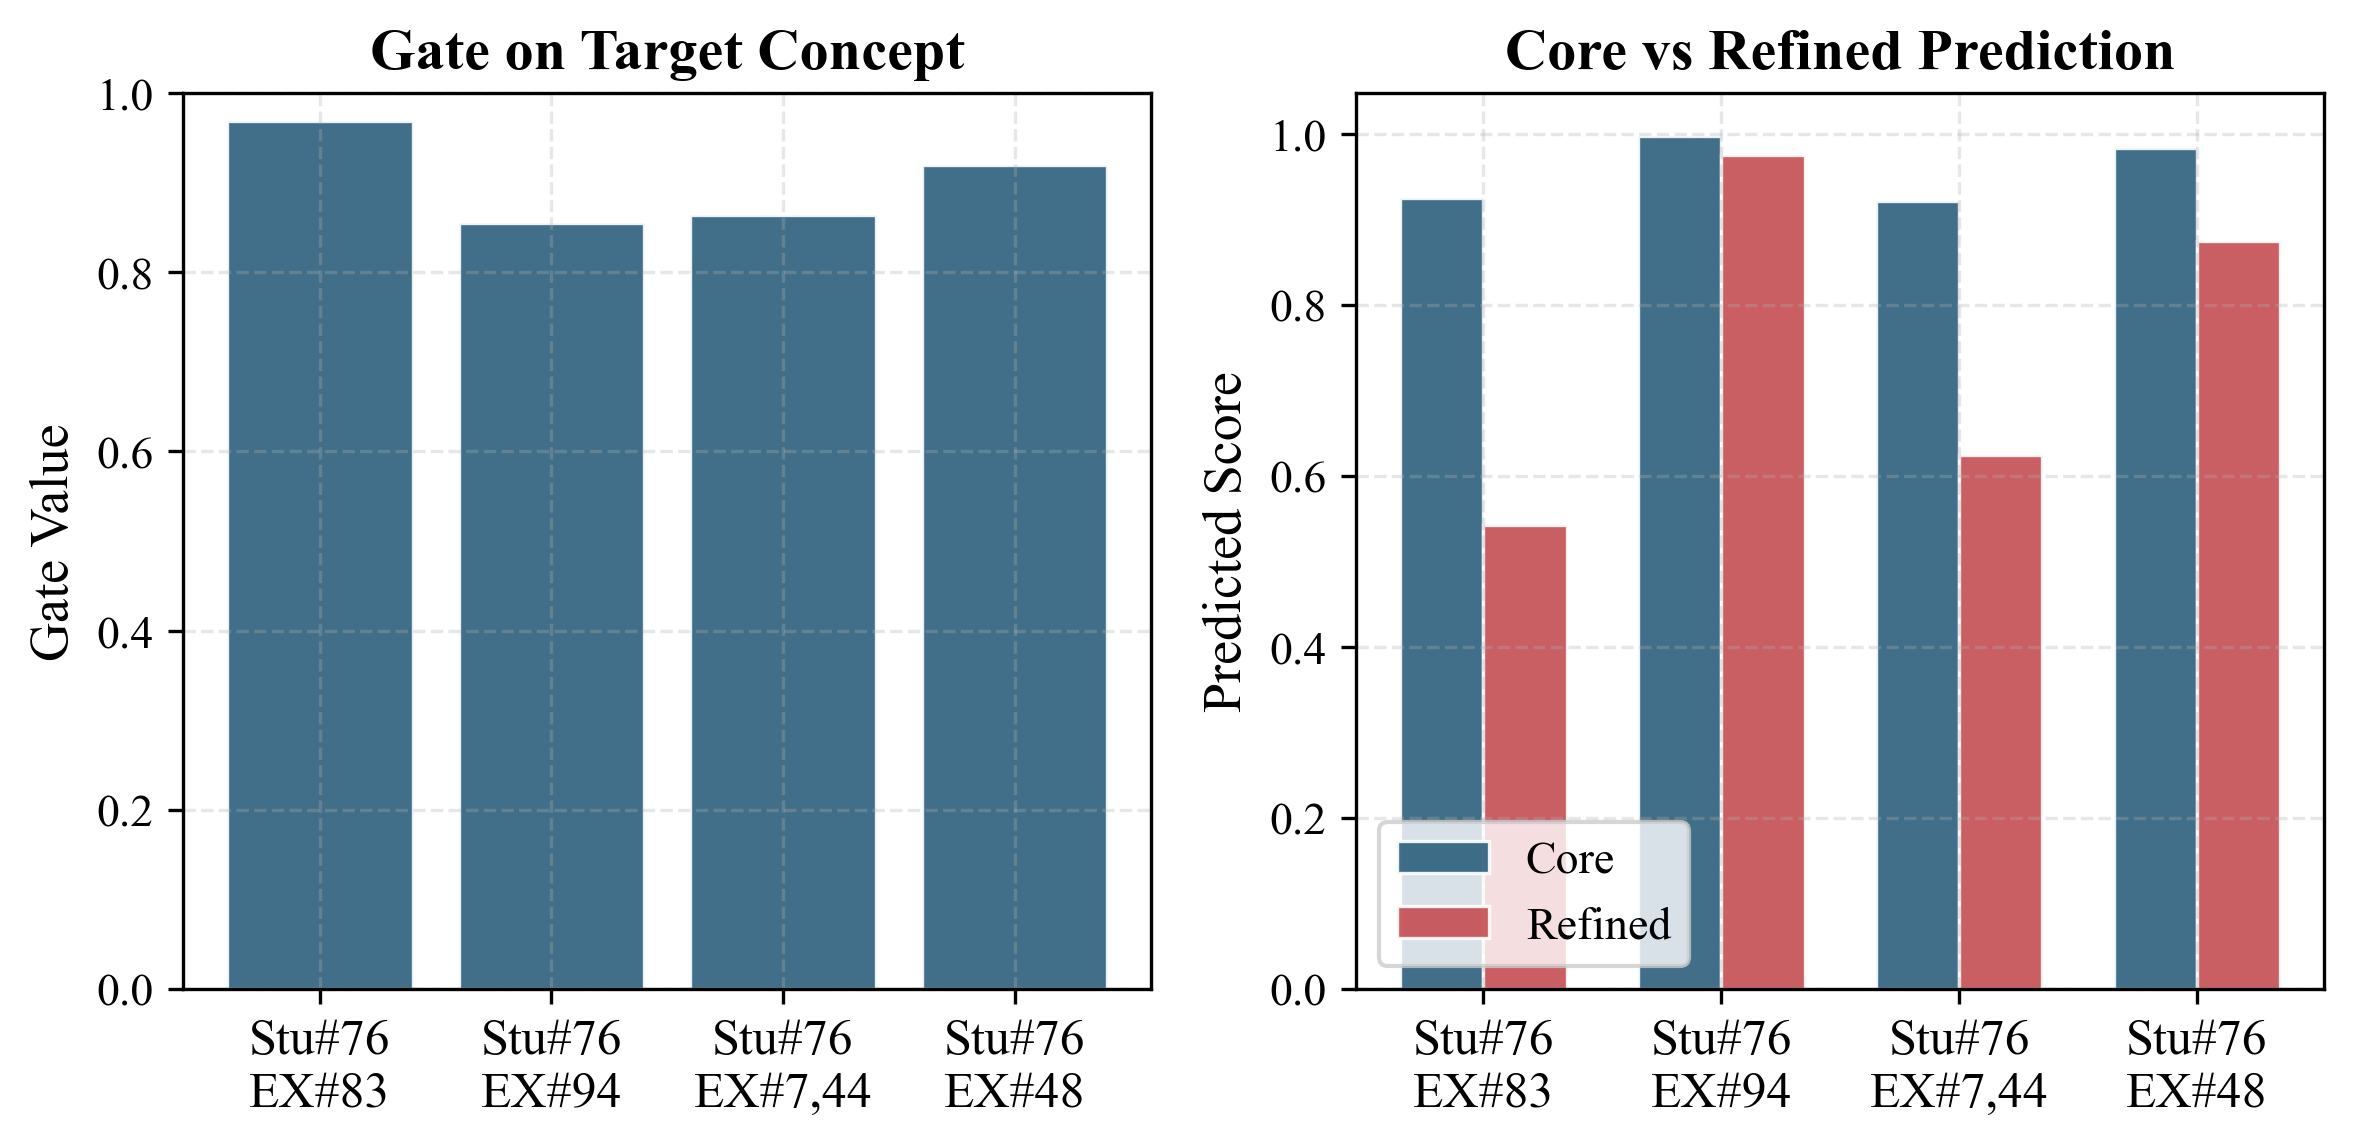
\includegraphics[width=\textwidth]{figure_bar_chart.png}
% \caption{Case study of \mymethod.}
% \label{fig:bar_case}
% \end{figure}

% Figure \ref{fig:bar_case} presents a case study of \mymethod, where gate value, core prediction, and refined prediction correspond to \(g_{i,j}\), \(\sigma(o_{i,j}^{\text{logit}})\), and \(\hat{y}_{i,j}\) in Section 4, respectively. For student \(u_{76}\), gate values across all four exercises exceed 0.85, indicating that behavioral fluency dominates the final predictions. Core predictions range from 0.92 to 0.99, which would lead traditional diagnosis to conclude that the student has mastered the relevant concepts. However, after the dynamic fusion gate incorporates behavioral fluency correction, final refined predictions drop sharply to 0.54 and 0.62 for exercises \(e_{83}\) and \(e_{744}\), respectively. This adjustment stems from behavioral characteristics in the student's historical interactions, including insufficient practice and low response consistency, which undermine fluency and trigger negative adjustments. This case validates the necessity of decoupling cognitive mastery from behavioral fluency. Relying solely on core predictions would substantially overestimate student performance, whereas incorporating behavioral fluency effectively distinguishes conceptual mastery from procedural fluency and delivers more accurate diagnostic conclusions.


% \subsection{Ablation Study}
% To deeply and rigorously evaluate the specific architectural contribution of each internal component, we systematically deconstructed our framework into three hierarchical variants, mathematically defined as follows:
% \begin{itemize}
%     \item \textbf{L1 (Only Fluency):} Strips away both the MTL behavioral encoder and the dynamic fusion gate. It treats "fluency" merely as a static, learnable embedding vector $E_{flu}$ without proxy constraints: $\hat{y} = \sigma(\text{MLP}(x_{mastery}) + W_{flu} E_{flu})$.
%     \item \textbf{L2 (Fluency + Behavior):} Re-introduces the explicit behavioral proxy features and MTL regularization, but lacks the dynamic fusion gate, forcing the network to rely on simple static concatenation: $\hat{y} = \sigma(\text{MLP}([x_{mastery} \parallel z]))$.
%     \item \textbf{L3 (Full \mymethod):} The complete, state-of-the-art framework equipped with both the structured MTL encoder and the adaptive dynamic fusion gate as mathematically defined in Equations 10, 11, and 12.
% \end{itemize}

% As thoroughly detailed in Table \ref{tab:ablation}, L1 establishes a solid, respectable baseline. Transitioning to L2 provides a marginal but consistent improvement in Accuracy, confirming the baseline utility of explicit behavioral encoding. However, the definitive, statistical leap in both AUC (0.9609) and minimized RMSE (0.2713) is observed exclusively in L3.

% Furthermore, Figure \ref{fig:ablation_bar} provides a clear, quantitative visual comparative analysis of the performance metrics across these variants. It explicitly highlights the step-wise performance gains achieved. This proves that while capturing behavioral features is undeniably important, the \textit{method} of fusing them with cognitive mastery is the true architectural bottleneck. Static fusion treats all questions identically, leading to severe feature dilution; the dynamic fusion gate successfully learns an item-aware routing mechanism.

% \begin{table}[t]
% \centering
% \caption{Hierarchical Ablation Study on Model Architecture.}
% \label{tab:ablation}
% \resizebox{0.8\columnwidth}{!}{
% \begin{tabular}{@{}lcccc@{}}
% \toprule
% \textbf{Model Variant} & \textbf{Gate Config} & \textbf{AUC} & \textbf{Accuracy} & \textbf{RMSE} \\ \midrule
% L1: Only Fluency       & w/o Gate             & 0.9602       & 0.8656            & 0.2815 \\
% L2: Fluency + Behavior & w/o Gate             & 0.9603       & 0.8696            & 0.2792 \\
% \textbf{L3: Full Model} & \textbf{w/ Gate}     & \textbf{0.9609} & \textbf{0.8747} & \textbf{0.2713} \\ \bottomrule
% \end{tabular}
% }
% \end{table}

% \begin{figure}[t]
% \centering
% \includegraphics[width=\columnwidth]{ablation_results_bar_chart.png}
% \caption{Performance comparison of different model variants in the ablation study. The full \mymethod\ framework (L3) achieves the highest AUC and Accuracy while minimizing the RMSE through its dynamic gating mechanism.}
% \label{fig:ablation_bar}
% \end{figure}


% \subsection{Case Study and Interpretability Analysis (RQ3)}
% A primary, overriding motivation for developing the \mymethod\ framework is to transition EDM from black-box correctness predictions to highly transparent, high-resolution cognitive profiling. To conclusively address \textbf{RQ3}, we conduct a qualitative, visual analysis focusing on the decoupling of cognitive states and the internal mathematical activation of the dynamic fusion gate.

% \subsubsection{Decoupling Mastery and Fluency (Radar Profiles):}
% Traditional CDMs structurally output a single scalar value per knowledge point. Figure \ref{fig:radar_case} illustrates a comparative diagnostic profile for two specific students (Student\#1 and Student\#2) across five distinct knowledge points (labeled A to E, representing domains such as Arithmetic, Fractions, Geometry, Algebra, and Probability).

% As clearly shown in Figure \ref{fig:radar_case}(a), the standard NCDM evaluates Student\#1 as strictly and globally superior to Student\#2 across all domains. From a practical pedagogical standpoint, this flat assessment would prompt an educator or an ITS algorithm to blindly assign extensive remedial conceptual lectures to Student\#2.

% However, when these identical interaction logs are evaluated through our decoupled \mymethod\ framework (Figure \ref{fig:radar_case}b), a highly nuanced, actionable reality emerges. The model successfully decouples the profile, revealing that Student\#1 and Student\#2 actually share highly comparable, fundamental \textit{Mastery} levels on core concepts (particularly domains A, B, and C). The severe performance disparity observed originally stems almost entirely from the \textit{Fluency} dimension (the procedural inability to execute the task quickly under testing conditions). In a real-world tutoring system, this dictates an entirely different, optimized intervention: Student\#2 requires targeted, time-constrained practice exercises to build problem-solving fluency, rather than enduring redundant theoretical retraining.

% \begin{figure}[t]
% \centering
% \includegraphics[width=0.9\textwidth]{figure_radar.png}
% \caption{Comparative diagnostic profiles. (a) Standard NCDM yields a single, entangled mastery metric. (b) \mymethod\ successfully decouples the cognitive state, revealing nuanced differences in behavioral fluency despite similar conceptual mastery.}
% \label{fig:radar_case}
% \end{figure}

% \subsubsection{Dynamic Gate Adaptation (Numerical Walkthrough \& Bar Charts):}
% Figure \ref{fig:bar_case} vividly illustrates the model's internal routing mechanism for two distinct students across two distinct knowledge points (KP\#79 and KP\#82). The left panel explicitly demonstrates that the gate value is highly variable and entirely item-aware. The dynamic gate essentially functions as an intelligent cognitive attention mechanism.

% To provide a concrete numerical walkthrough: consider Student\#2827 on KP\#79 (a highly procedural task, e.g., "Simplifying Fractions"). The model extracts a latent fluency score $z_{flu} = 0.21$ (indicating poor procedural familiarity). Because the question is highly procedural, the dynamic gate $g$ activates at a high level of $0.85$. Following Equation 11, the residual adjustment applied to the logit is mathematically $\gamma \cdot 0.85 \cdot (0.21 - 0.5) \cdot 4.0 \approx -0.98$. This mathematically executes a sharp, severe penalty on the final prediction logit (as seen in the deep orange bar extending downwards in the right panel).

% Conversely, for KP\#82 (a deep conceptual task, e.g., "Understanding Limits"), the gate activation drops significantly ($\approx 0.3$), dampening the $(flu-0.5)$ penalty and forcing the model to disregard procedural slips and rely heavily on the fundamental cognitive mastery branch. This definitively proves that \mymethod\ effectively learns a self-adaptive routing strategy.

% \begin{figure}[t]
% \centering
% \includegraphics[width=\textwidth]{figure_bar_chart.jpg}
% \caption{Visualization of Dynamic Gate Adaptation. The left panel shows the dynamic gating values ($g$). The right panel illustrates how the gate dynamically scales the prediction logits based on whether the question tests a ``Core'' or ``Refined Core'' concept.}
% \label{fig:bar_case}
% \end{figure}

\section{Conclusion}
In this paper, we proposed \mymethod, a dual-stream CD framework that disentangles student cognitive states into mastery and behavioral fluency dimensions. Unlike existing CDMs that rely solely on binary correctness, \mymethod\ captures behavioral fluency through three proxy features, including exposure intensity, empirical accuracy, and response consistency. A dynamic fusion gate adaptively integrates this behavioral signal with cognitive mastery from any backbone CDM, enabling fluency-aware correction. The multi-task objective jointly optimizes the primary prediction and three auxiliary reconstruction losses to preserve behavioral information. Extensive experiments on six benchmark datasets clearly demonstrate both the effectiveness and generalizability of our \mymethod.

% In this paper, we proposed a novel and highly interpretable Multi-Task Learning framework that successfully bridges the historical gap between deep cognitive modeling and practical behavioral dynamics. To directly overcome the critical limitations of traditional unidimensional models, our framework explicitly decouples students' cognitive profiles into distinct \textit{Mastery} and \textit{Fluency} dimensions. By introducing key behavioral proxy features (Opportunity, Accuracy Prior, Stability) and engineering an intelligent dynamic fusion gate, our plug-and-play module universally and significantly enhances the predictive performance of all tested baseline models across diverse real-world educational datasets.
% Future work will explore extending this decoupled framework to sequential \textit{Knowledge Tracing} (KT) architectures to model temporal dynamics and integrate richer multimodal behavioral signals, such as eye-tracking or video-based engagement metrics.

\begin{credits}
\subsubsection{\discintname}
The authors have no competing interests to declare that are relevant to the content of this article.
\end{credits}

% ---- Bibliography ----

\bibliographystyle{splncs04}
\bibliography{refs}

% \begin{thebibliography}{99}

% % ==================================================
% % 1. 经典预测与推荐模型
% % ==================================================
% \bibitem{thai2010recommender}
% Nguyen Thai-Nghe, Lucas Drumond, Artus Krohn-Grimberghe, and Lars Schmidt-Thieme, ``Recommender system for predicting student performance,'' \textit{Procedia Computer Science}, vol. 1, no. 2, pp. 2811--2819, 2010.

% % ==================================================
% % 2. 传统统计学与心理测量学基线 (Baselines: IRT, MIRT, DINA)
% % ==================================================
% \bibitem{fan1998item}
% Xitao Fan, ``Item response theory and classical test theory: An empirical comparison of their item/person statistics,'' \textit{Educational and Psychological Measurement}, vol. 58, no. 3, pp. 357--381, 1998.

% \bibitem{junker2001cognitive}
% Brian W. Junker and Klaas Sijtsma, ``Cognitive assessment models with few assumptions, and connections with nonparametric item response theory,'' \textit{Applied Psychological Measurement}, vol. 25, no. 3, pp. 258--272, 2001.

% \bibitem{reckase2009multidimensional}
% Mark D. Reckase, ``Multidimensional item response theory models,'' in \textit{Multidimensional Item Response Theory}, Springer, pp. 79--112, 2009.

% \bibitem{delatorre2009dina}
% Jimmy De La Torre, ``Dina model and parameter estimation: A didactic,'' \textit{Journal of Educational and Behavioral Statistics}, vol. 34, no. 1, pp. 115--130, 2009.

% \bibitem{delatorre2011generalized}
% Jimmy De La Torre, ``The generalized dina model framework,'' \textit{Psychometrika}, vol. 76, no. 2, pp. 179--199, 2011.

% \bibitem{linden2000computerized}
% Wim J. Van der Linden, Cees A. W. Glas, et al., \textit{Computerized adaptive testing: Theory and practice}, Springer, vol. 13, 2000.

% % ==================================================
% % 3. 深度学习与深度认知诊断基线 (Baselines: NCDM, NeuralCD, DKT)
% % ==================================================
% \bibitem{piech2015deep}
% Chris Piech, Jonathan Bassen, Jonathan Huang, Surya Ganguli, Mehran Sahami, Leonidas J. Guibas, and Jascha Sohl-Dickstein, ``Deep knowledge tracing,'' \textit{Advances in Neural Information Processing Systems}, vol. 28, 2015.

% \bibitem{liu2018fuzzy}
% Qi Liu, Runze Wu, Enhong Chen, Guandong Xu, Yu Su, Zhigang Chen, and Guoping Hu, ``Fuzzy cognitive diagnosis for modelling examinee performance,'' \textit{ACM Transactions on Intelligent Systems and Technology (TIST)}, vol. 9, no. 4, pp. 1--26, 2018.

% \bibitem{wang2020neural}
% Fei Wang, Qi Liu, Enhong Chen, Zhenya Huang, Yuying Chen, Yu Yin, Zai Huang, and Shijin Wang, ``Neural cognitive diagnosis for intelligent education systems,'' in \textit{Proceedings of the AAAI Conference on Artificial Intelligence}, vol. 34, no. 04, pp. 6153--6161, 2020.

% \bibitem{wang2022neuralcd}
% Fei Wang, Qi Liu, Enhong Chen, Zhenya Huang, Yu Yin, Shijin Wang, and Yu Su, ``Neuralcd: a general framework for cognitive diagnosis,'' \textit{IEEE Transactions on Knowledge and Data Engineering}, vol. 35, no. 8, pp. 8312--8327, 2022.

% \bibitem{wang2023dynamic}
% Fei Wang, Zhenya Huang, Qi Liu, Enhong Chen, Yu Yin, Jianhui Ma, and Shijin Wang, ``Dynamic cognitive diagnosis: An educational priors-enhanced deep knowledge tracing perspective,'' \textit{IEEE Transactions on Learning Technologies}, vol. 16, no. 3, pp. 306--323, 2023.

% \bibitem{wang2023review}
% Yu Wang, Mengxia Zhu, Shanghui Yang, Xuesong Lu, and Aoying Zhou, ``Review and performance comparison of deep knowledge tracing models,'' \textit{Journal of Software}, vol. 34, no. 3, pp. 1365--1395, 2023.

% % ==================================================
% % 4. 行为、情感状态与解耦动态
% % ==================================================
% \bibitem{wang2024boosting}
% Shanshan Wang, Zhen Zeng, Xun Yang, Ke Xu, and Xingyi Zhang, ``Boosting neural cognitive diagnosis with student's affective state modeling,'' in \textit{Proceedings of the AAAI Conference on Artificial Intelligence}, vol. 38, no. 1, pp. 620--627, 2024.

% \bibitem{zhang2025cognitive}
% Yuhong Zhang, Zhihao Lin, Chenyang Bu, Kui Yu, Xuegang Hu, and Xindong Wu, ``A cognitive diagnosis model with nonlinear dependence between students and exercises,'' \textit{IEEE Transactions on Computational Social Systems}, pp. 1--12, 2025.

% \bibitem{smith1994misconceptions}
% John P. Smith III, Andrea A. DiSessa, and Jeremy Roschelle, ``Misconceptions reconceived: A constructivist analysis of knowledge in transition,'' \textit{The Journal of the Learning Sciences}, vol. 3, no. 2, pp. 115--163, 1994.

% % ==================================================
% % 5. 知识追踪的最新图模型与增强框架 (SOTA CDMs 2025/2026)
% % ==================================================
% \bibitem{zhang2021gkt}
% Junrui Zhang, Yun Mo, Changzhi Chen, and Xiaofeng He, ``Gkt-cd: Make cognitive diagnosis model enhanced by graph-based knowledge tracing,'' in \textit{2021 International Joint Conference on Neural Networks (IJCNN)}, IEEE, pp. 1--8, 2021.

% \bibitem{su2022graph}
% Yu Su, Zeyu Cheng, Jinze Wu, Yanmin Dong, Zhenya Huang, Le Wu, Enhong Chen, Shijin Wang, and Fei Xie, ``Graph-based cognitive diagnosis for intelligent tutoring systems,'' \textit{Knowledge-Based Systems}, vol. 253, p. 109547, 2022.

% \bibitem{zhou2024predictive}
% Hanqi Zhou, Robert Bamler, Charley Wu, and Alvaro Tejero-Cantero, ``Predictive, scalable and interpretable knowledge tracing on structured domains,'' in \textit{International Conference on Learning Representations}, vol. 2024, pp. 35609--35622, 2024.

% \bibitem{huang2024xkt}
% Chang-Qin Huang, Qiong-Hao Huang, Xiaodi Huang, Hua Wang, Ming Li, Kwei-Jay Lin, and Yi Chang, ``Xkt: toward explainable knowledge tracing model with cognitive learning theories for questions of multiple knowledge concepts,'' \textit{IEEE Transactions on Knowledge and Data Engineering}, vol. 36, no. 11, pp. 7308--7325, 2024.

% \bibitem{ma2024hd}
% Haiping Ma, Yong Yang, Chuan Qin, Xiaoshan Yu, Shangshang Yang, Xingyi Zhang, and Hengshu Zhu, ``Hd-kt: advancing robust knowledge tracing via anomalous learning interaction detection,'' in \textit{Proceedings of the ACM Web Conference 2024}, pp. 4479--4488, 2024.

% \bibitem{dong2025knowledge}
% Zhiang Dong, Jingyuan Chen, and Fei Wu, ``Knowledge is power: Harnessing large language models for enhanced cognitive diagnosis,'' in \textit{Proceedings of the AAAI Conference on Artificial Intelligence}, vol. 39, no. 1, pp. 164--172, 2025.

% \bibitem{yang2025endowing}
% Shangshang Yang, Linrui Qin, Xiaoshan Yu, Ziwen Wang, Xueming Yan, Haiping Ma, and Ye Tian, ``Endowing interpretability for neural cognitive diagnosis by efficient kolmogorov-arnold networks,'' in \textit{Proceedings of the Thirty-Fourth International Joint Conference on Artificial Intelligence}, pp. 7894--7903, 2025.

% \bibitem{zhao2025multi}
% Guanhao Zhao, Zhenya Huang, Cheng Cheng, Yan Zhuang, Qingyang Mao, Xin Li, Shijin Wang, and Enhong Chen, ``Multi-perspective consolidation enhanced cognitive diagnosis via conditional diffusion model,'' in \textit{Proceedings of the AAAI Conference on Artificial Intelligence}, vol. 39, no. 1, pp. 1174--1182, 2025.

% \bibitem{zhang2026knowledge}
% Miao Zhang, Huihuan Li, Lele Zheng, Shunfeng Tan, Chao Yang, Kui Xiao, Zhifang Huang, and Zhifei Li, ``Knowledge concept cold-start approach for cognitive diagnosis,'' \textit{Neurocomputing}, vol. 672, p. 132770, 2026.

% \bibitem{liu2026knowledge}
% Chengfeng Liu, Jianrui Chen, Zhihui Wang, and Longjiang Guo, ``Knowledge graph-based cognitive learning with multi-fact reasoning,'' \textit{Neural Networks}, p. 108747, 2026.

% \end{thebibliography}

\end{document}
